% Options for packages loaded elsewhere
\PassOptionsToPackage{unicode}{hyperref}
\PassOptionsToPackage{hyphens}{url}
\PassOptionsToPackage{dvipsnames,svgnames,x11names}{xcolor}
%
\documentclass[
  letterpaper,
  DIV=11,
  numbers=noendperiod]{scrartcl}

\usepackage{amsmath,amssymb}
\usepackage{setspace}
\usepackage{iftex}
\ifPDFTeX
  \usepackage[T1]{fontenc}
  \usepackage[utf8]{inputenc}
  \usepackage{textcomp} % provide euro and other symbols
\else % if luatex or xetex
  \usepackage{unicode-math}
  \defaultfontfeatures{Scale=MatchLowercase}
  \defaultfontfeatures[\rmfamily]{Ligatures=TeX,Scale=1}
\fi
\usepackage{lmodern}
\ifPDFTeX\else  
    % xetex/luatex font selection
\fi
% Use upquote if available, for straight quotes in verbatim environments
\IfFileExists{upquote.sty}{\usepackage{upquote}}{}
\IfFileExists{microtype.sty}{% use microtype if available
  \usepackage[]{microtype}
  \UseMicrotypeSet[protrusion]{basicmath} % disable protrusion for tt fonts
}{}
\makeatletter
\@ifundefined{KOMAClassName}{% if non-KOMA class
  \IfFileExists{parskip.sty}{%
    \usepackage{parskip}
  }{% else
    \setlength{\parindent}{0pt}
    \setlength{\parskip}{6pt plus 2pt minus 1pt}}
}{% if KOMA class
  \KOMAoptions{parskip=half}}
\makeatother
\usepackage{xcolor}
\ifLuaTeX
  \usepackage{luacolor}
  \usepackage[soul]{lua-ul}
\else
  \usepackage{soul}
  
\fi
\setlength{\emergencystretch}{3em} % prevent overfull lines
\setcounter{secnumdepth}{-\maxdimen} % remove section numbering
% Make \paragraph and \subparagraph free-standing
\ifx\paragraph\undefined\else
  \let\oldparagraph\paragraph
  \renewcommand{\paragraph}[1]{\oldparagraph{#1}\mbox{}}
\fi
\ifx\subparagraph\undefined\else
  \let\oldsubparagraph\subparagraph
  \renewcommand{\subparagraph}[1]{\oldsubparagraph{#1}\mbox{}}
\fi


\providecommand{\tightlist}{%
  \setlength{\itemsep}{0pt}\setlength{\parskip}{0pt}}\usepackage{longtable,booktabs,array}
\usepackage{calc} % for calculating minipage widths
% Correct order of tables after \paragraph or \subparagraph
\usepackage{etoolbox}
\makeatletter
\patchcmd\longtable{\par}{\if@noskipsec\mbox{}\fi\par}{}{}
\makeatother
% Allow footnotes in longtable head/foot
\IfFileExists{footnotehyper.sty}{\usepackage{footnotehyper}}{\usepackage{footnote}}
\makesavenoteenv{longtable}
\usepackage{graphicx}
\makeatletter
\def\maxwidth{\ifdim\Gin@nat@width>\linewidth\linewidth\else\Gin@nat@width\fi}
\def\maxheight{\ifdim\Gin@nat@height>\textheight\textheight\else\Gin@nat@height\fi}
\makeatother
% Scale images if necessary, so that they will not overflow the page
% margins by default, and it is still possible to overwrite the defaults
% using explicit options in \includegraphics[width, height, ...]{}
\setkeys{Gin}{width=\maxwidth,height=\maxheight,keepaspectratio}
% Set default figure placement to htbp
\makeatletter
\def\fps@figure{htbp}
\makeatother
% definitions for citeproc citations
\NewDocumentCommand\citeproctext{}{}
\NewDocumentCommand\citeproc{mm}{%
  \begingroup\def\citeproctext{#2}\cite{#1}\endgroup}
\makeatletter
 % allow citations to break across lines
 \let\@cite@ofmt\@firstofone
 % avoid brackets around text for \cite:
 \def\@biblabel#1{}
 \def\@cite#1#2{{#1\if@tempswa , #2\fi}}
\makeatother
\newlength{\cslhangindent}
\setlength{\cslhangindent}{1.5em}
\newlength{\csllabelwidth}
\setlength{\csllabelwidth}{3em}
\newenvironment{CSLReferences}[2] % #1 hanging-indent, #2 entry-spacing
 {\begin{list}{}{%
  \setlength{\itemindent}{0pt}
  \setlength{\leftmargin}{0pt}
  \setlength{\parsep}{0pt}
  % turn on hanging indent if param 1 is 1
  \ifodd #1
   \setlength{\leftmargin}{\cslhangindent}
   \setlength{\itemindent}{-1\cslhangindent}
  \fi
  % set entry spacing
  \setlength{\itemsep}{#2\baselineskip}}}
 {\end{list}}
\usepackage{calc}
\newcommand{\CSLBlock}[1]{\hfill\break\parbox[t]{\linewidth}{\strut\ignorespaces#1\strut}}
\newcommand{\CSLLeftMargin}[1]{\parbox[t]{\csllabelwidth}{\strut#1\strut}}
\newcommand{\CSLRightInline}[1]{\parbox[t]{\linewidth - \csllabelwidth}{\strut#1\strut}}
\newcommand{\CSLIndent}[1]{\hspace{\cslhangindent}#1}

\KOMAoption{captions}{tableheading}
\makeatletter
\@ifpackageloaded{caption}{}{\usepackage{caption}}
\AtBeginDocument{%
\ifdefined\contentsname
  \renewcommand*\contentsname{Table of contents}
\else
  \newcommand\contentsname{Table of contents}
\fi
\ifdefined\listfigurename
  \renewcommand*\listfigurename{List of Figures}
\else
  \newcommand\listfigurename{List of Figures}
\fi
\ifdefined\listtablename
  \renewcommand*\listtablename{List of Tables}
\else
  \newcommand\listtablename{List of Tables}
\fi
\ifdefined\figurename
  \renewcommand*\figurename{Figure}
\else
  \newcommand\figurename{Figure}
\fi
\ifdefined\tablename
  \renewcommand*\tablename{Table}
\else
  \newcommand\tablename{Table}
\fi
}
\@ifpackageloaded{float}{}{\usepackage{float}}
\floatstyle{ruled}
\@ifundefined{c@chapter}{\newfloat{codelisting}{h}{lop}}{\newfloat{codelisting}{h}{lop}[chapter]}
\floatname{codelisting}{Listing}
\newcommand*\listoflistings{\listof{codelisting}{List of Listings}}
\makeatother
\makeatletter
\makeatother
\makeatletter
\@ifpackageloaded{caption}{}{\usepackage{caption}}
\@ifpackageloaded{subcaption}{}{\usepackage{subcaption}}
\makeatother
\ifLuaTeX
  \usepackage{selnolig}  % disable illegal ligatures
\fi
\usepackage{bookmark}

\IfFileExists{xurl.sty}{\usepackage{xurl}}{} % add URL line breaks if available
\urlstyle{same} % disable monospaced font for URLs
\hypersetup{
  colorlinks=true,
  linkcolor={blue},
  filecolor={Maroon},
  citecolor={Blue},
  urlcolor={Blue},
  pdfcreator={LaTeX via pandoc}}

\author{}
\date{}

\begin{document}

\setstretch{1.5}
\section{Introduction}\label{introduction}

\subsection{Background}\label{background}

How does the brain efficiently process the overwhelming amount of
sensory input that it receives from a constantly changing and uncertain
environment? According to the predictive coding (PC) framework, the
brain's key solution is to actively predict incoming sensory input based
on past observations and to prioritize the processing of unpredicted
sensory information (Huang and Rao 2011). PC envisions the brain as a
prediction machine, where predictions are made through prior experience
or expectation. These predictions are compared to the actual sensory
input, and the difference, known as prediction error, is used to refine
the internal model of the environment and orient attention towards
unexpected features of the input. This allows the brain to minimize the
prediction error and allocate its finite resources more efficiently
(Vinck, Uran, and Canales-Johnson 2022).

Predictive coding is generally thought to be implemented by the cortex.
Indeed, the mammalian cortex is organized hierarchically, with lower
level areas processing more basic sensory features and higher areas
integrating this information into more complex representations (Felleman
and Van Essen 1991). Visual cortex is a prime example of this hierarchy,
with primary visual cortex (V1) processing simple visual features like
contrast and edges and higher visual areas (e.g.~V2, V4) extracting more
complex features of stimuli like texture and shape (Huff, Mahabadi, and
Tadi 2018). The hierarchy of cortical processing allows the brain to
make predictions at multiple levels of abstraction and compare these
predictions to the actual sensory input. According to PC, communication
between hierarchical cortical areas occurs through feedforward (FF) and
feedback (FB) connections. FB projections involve top-down propagation
of prediction from higher to lower-level areas, while FF projections
involve bottom-up assembly of sensory input and prediction error from
lower to higher-level areas to update the internal model. FF and FB
connections have distinct laminar origins and targets within the cortex.
FF connections mainly originate from layers 3 and 5 (of lower areas) and
target the layer 4 (of higher area). On the other hand, FB connections
arise from layers 2 and 6 (of higher areas) and target all layers except
for layer 4 (of lower areas) (Vinck, Uran, and Canales-Johnson 2022).

Prominent studies in primates visual systems (Van Kerkoerle et al. 2014)
suggest neural oscillations might play an important role in
communication between cortical regions through FF-FB connections. The
studies found that FF propagation is associated with gamma-band
oscillations (30--100 Hz), while FB propagation involves alpha-band
oscillations (8--12 Hz). Similarly, a study on mice (Aggarwal et al.
2022) vision revealed FF waves in the 30--50 Hz range and FB waves in
the 3-6 Hz range, where the phase of the FB oscillations modulated the
amplitude of the FF oscillations. However, this was the only study on
mice, to the best of my knowledge, that has investigated the FF-FB waves
in the visual system. Additionally, the study utilized a simple visual
stimulus that did not involve any prediction and higher-level cognitive
processes.

The mouse visual system offers several advantages for studying
predictive coding. The simpler and well-studied visual processing
hierarchy in mice allows for more straightforward analysis of neural
data. Genetic manipulation tools in mice also provide unique
opportunities to explore cortical micro-circuitry and manipulate neural
pathways, which is challenging in primates. Additionally, mouse studies
are more cost-effective and logistically feasible compare to primates,
making them an attractive model for large-scale explorations of complex
brain functions like predictive coding.

The International Brain Laboratory (IBL) (Benson et al. 2023) provides
an extensive open-access dataset recorded from more than 100 mice
trained to perform a perceptual decision-making task. In this task, mice
are presented with a visual stimulus of controlled contrast and are
required to move the stimulus to the center of the screen using a
steering wheel. The stimulus appears on the right or left side of the
screen, with a fixed probability for blocks of trials to create a
predictable pattern. Yet, these bias blocks change unpredictably,
requiring the mice to constantly update their predictions and internal
model of the environment. Therefore, this sophisticated experimental
paradigm provides a valuable opportunity to study the neural
implementation of predictive coding.

\subsection{Current project}\label{current-project}

To date, IBL researchers have primarily focused on detecting, sorting,
and analyzing action potentials and firing rates, without prioritizing a
specific brain region or cognitive process. The overarching goal of the
current project is to go beyond their data-driven analyses and to use
the IBL dataset as a benchmark to study the neural implementation of
predictive coding in the mammalian brain. In this perspective, we were
particularly interested in local field potentials (LFP) and oscillatory
electrophysiological signals in the theta (typically, between 2 to 7
Hz), alpha (7 to 15 Hz), beta (15 to 40 Hz) and gamma (40 to 200Hz).
Until recently, LFPs recorded in the IBL context have been left almost
unexplored and the analysis of LFP signals produced by Neuropixel probes
(as used by all IBL experiments) has received limited attention (Windolf
et al. 2023). In other words, the current project represents a first
step towards unlocking the great potential of the IBL dataset to
constrain theories of predictive coding and brain communication through
oscillations.

Thus, my primary goal was to assess the quality and usability of IBL LFP
data through a careful development of preprocessing pipelines and the
comparison of different artifact detection and signal re-referencing
methods. My second goal was to confirm that a core principle of
communication through oscillations could be observed in the dataset. To
reach this goal, I performed the following analysis: 1) The inter trial
phase coherence (ITC) analysis, as it reflects the degree of temporal
synchronization in response to sensory stimuli. 2) Time frequency
analysis to examine the dynamic change in high and low frequency ranges
over time, as they are indicators of FF and Fb communications,
respectively. 3) Analyzing phase amplitude coupling (PAC) in order to
quantify the degree to which the phase of low frequency oscillations
modulates the amplitude of high frequency waves. Growing evidence claim
this cross frequency interaction facilitate communication within the
brain during sensory processing (Bonnefond and Jensen 2015; Seymour,
Rippon, and Kessler 2017).

\section{Methods}\label{methods}

\subsection{Data recording details}\label{data-recording-details}

\subsubsection{Task detail}\label{task-detail}

In the IBL task (Figure 1a,b), head-fixed mice had to move a visual
stimulus to the center by turning a wheel with their front paws. At the
start of each trial, the mouse was required to refrain from moving the
wheel for a quiescence period lasting between 400 and 700 milliseconds.
After this period, a visual stimulus (Gabor patch) appeared on either
the left or right side of the screen accompanied by a 100-millisecond
tone (5 kHz sine wave). If the mouse correctly moved the stimulus to the
center by turning the wheel over 35°, it received a 3 µL water reward.
Incorrect responses or failing to respond within 60 seconds resulted in
a 500-millisecond burst of white noise and a timeout (Benson et al.
2023). As shown in Figure 1c, mice typically responded quickly mainly
within 2 seconds. The stimulus is always presented for the first 1
second regardless of response time (RT). RT is defined as the time after
stimulus when the wheel rotation exceeds the threshold.

The experiment began with 90 unbiased trials where the stimulus appeared
equally on both sides. The stimulus contrast levels were presented in a
ratio of {[}2:2:2:2:1{]} for contrasts {[}100\%, 25\%, 12.5\%, 6\%,
0\%{]}. After this initial block, trials were organized into biased
blocks where the likelihood of the stimulus appearing on one side was
fixed at 20\% for the left and 80\% for the right in ``right blocks'' or
vice versa in ``left blocks.'' These blocks consisted of 20 to 100
trials determined by a truncated geometric distribution with stimulus
contrast levels ratio identical to those in the unbiased block. In 0\%
contrast trials where no stimulus was visible, the side assignment
followed the block bias (e.g., right side for right blocks) (Benson et
al. 2023).

\begin{figure}

{\centering 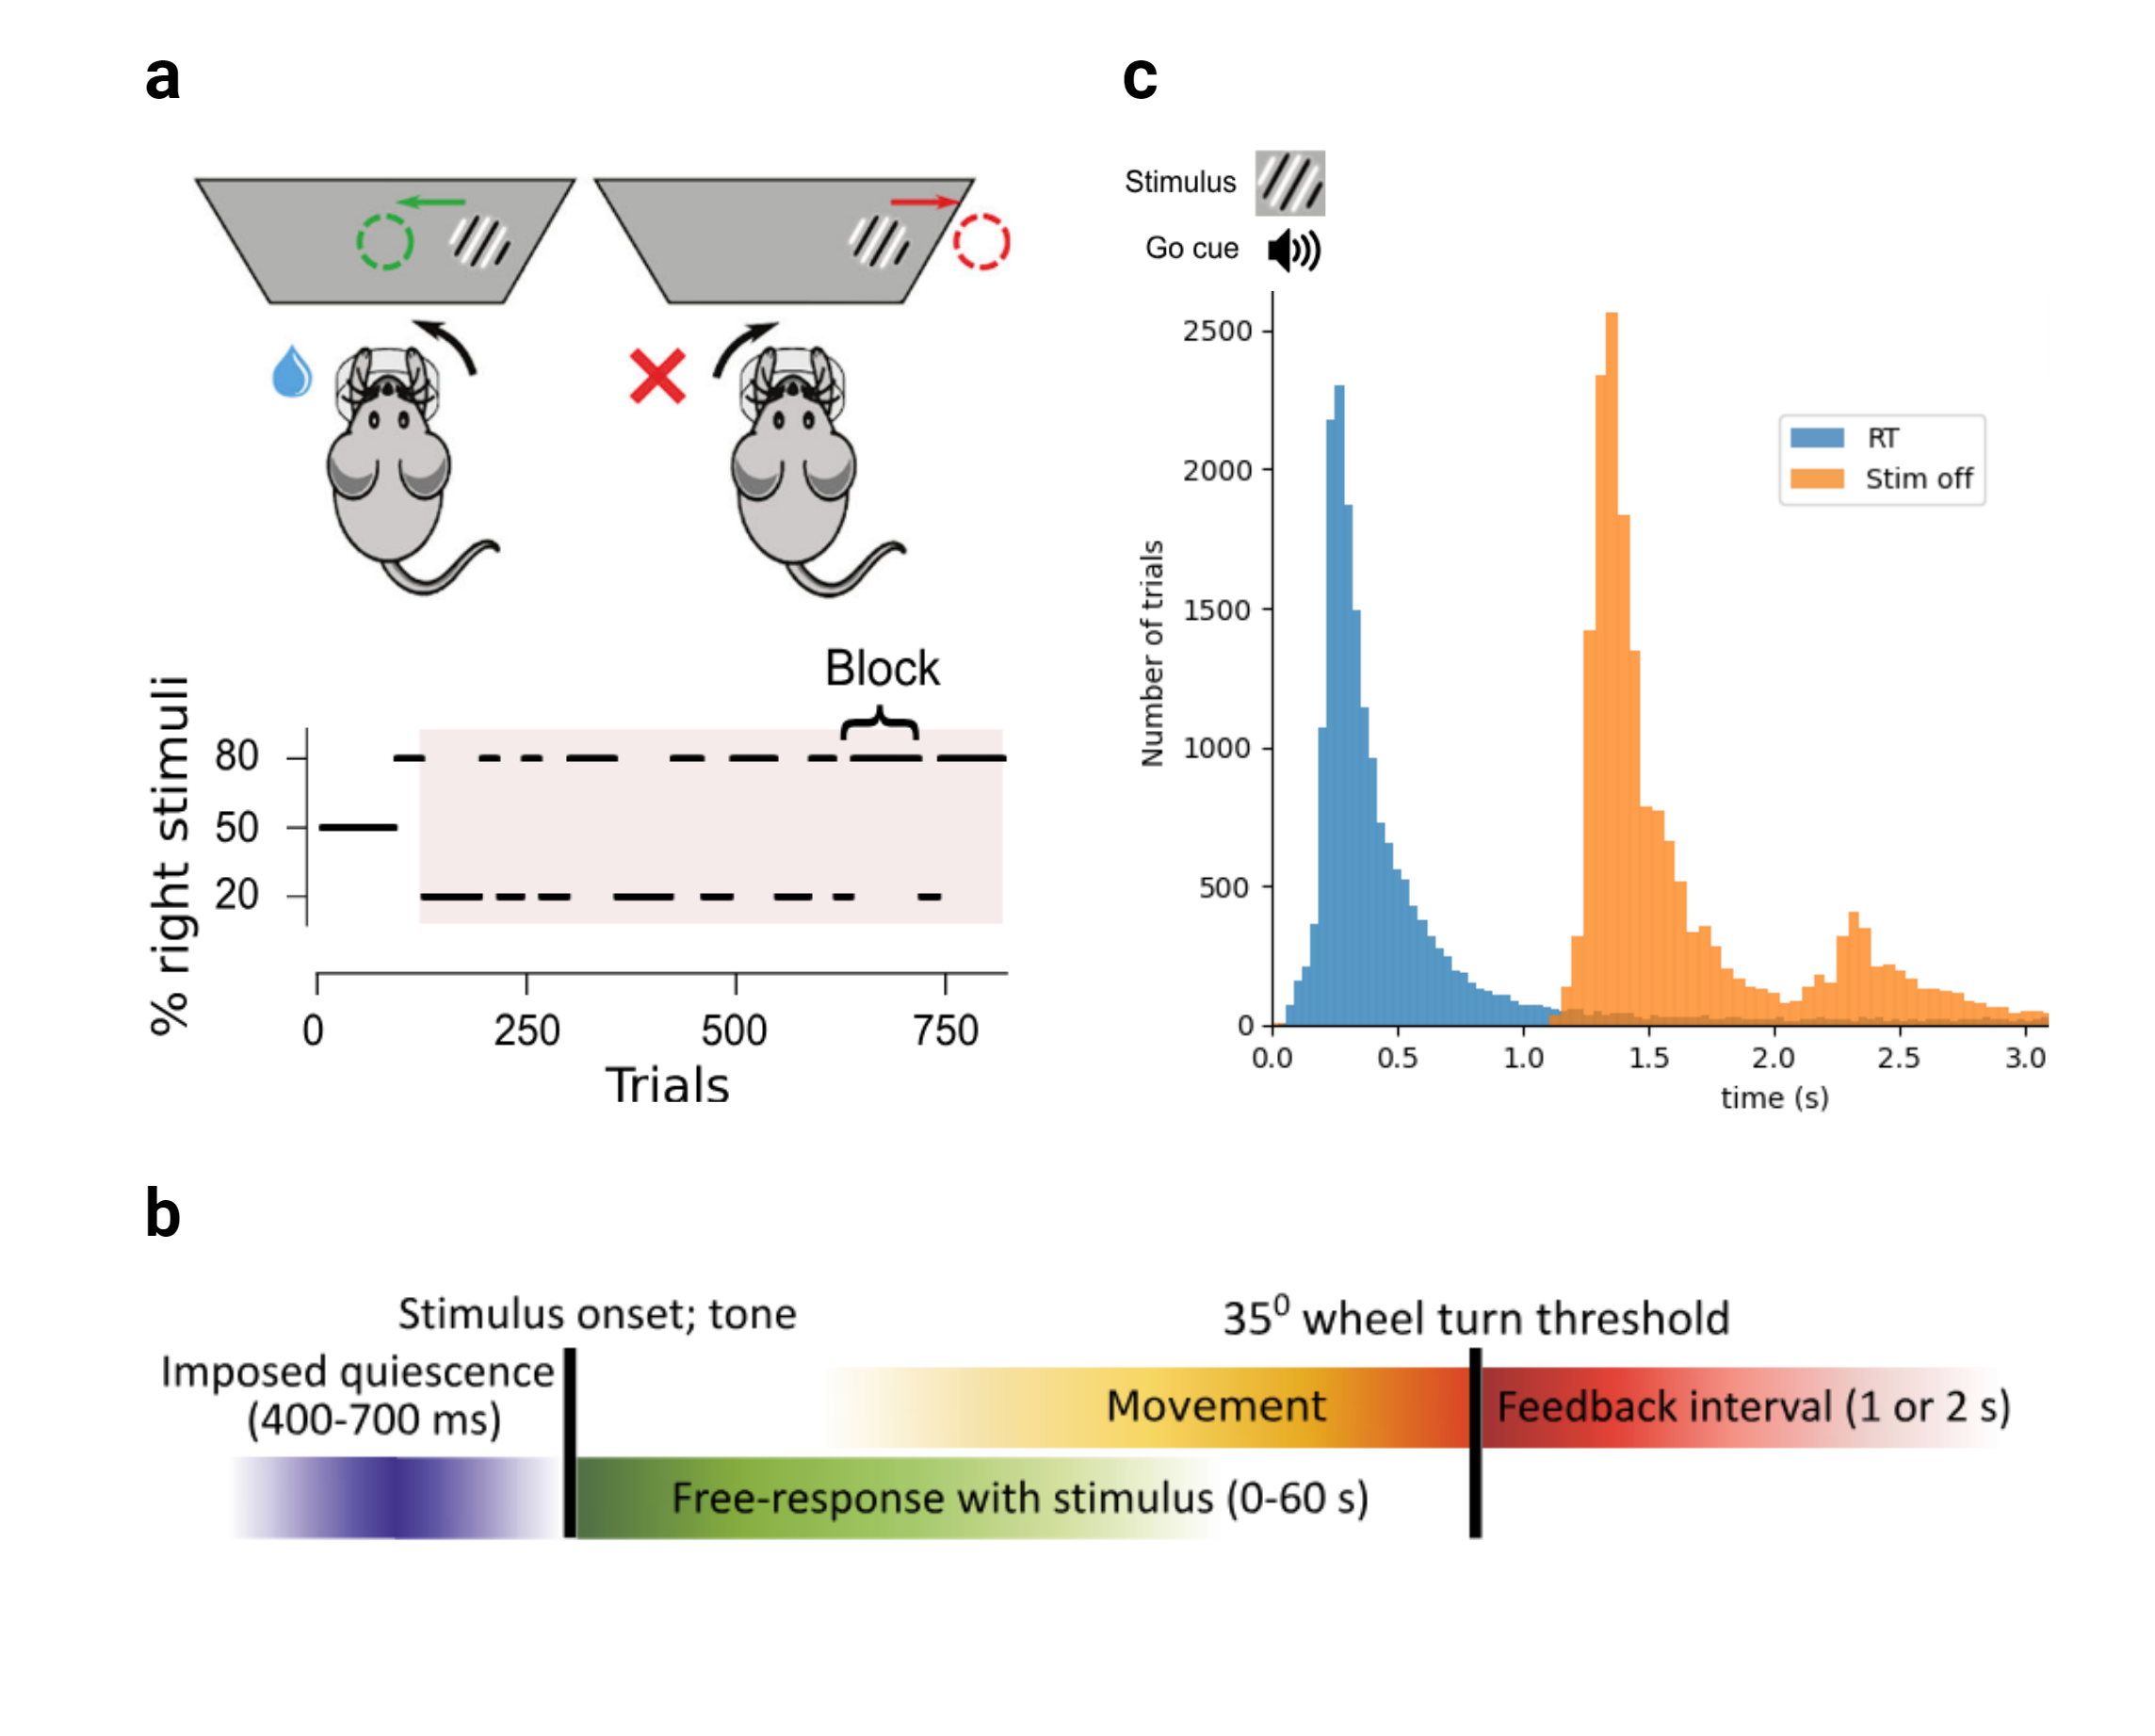
\includegraphics[width=6.46875in,height=\textheight]{images/task.png}

}

\caption{\textbf{International Brain Laboratory (IBL) task. a)} Example
session block diagram and IBL task. Each block of consecutive trials
after 90 trials varied the probability of the stimulus being on the
right side. \textbf{B)} A timeline of the main events and variables of
the IBL task. After a quiescence period, stimulus appears on screen
alongside a go cue tone. Mice had to bring the stimulus to the center by
turning the wheel. When the wheel rotation reaches the threshold 35 ° or
after 60 s of no response, positive or negative feedback is provided
depending on the mice choice. (a) and (b) panels are extracted from
(Benson et al. 2023) . \textbf{C)} Distribution of response time (RT)
with color blue and stimulus offset time with color yellow relative to
stimulus onset. Note that there is always a stimulus presented for the
first 1 second even though the mice typically answer sooner.~}

\end{figure}%

\subsubsection{Electrophysiological
recording}\label{electrophysiological-recording}

The neural recordings were conducted using Neuropixel probes with 384
recording channels and 960 low-impedance sites on a single shank (Benson
et al. 2023). Neuropixel probes are advanced silicon-based neural
recording devices designed for high-density recording of neural activity
across large populations of neurons with precise spatial and temporal
resolution (Jun et al. 2017). Data are collected from 267 brain regions
by inserting 547 Neuropixel probes covering most of the left hemisphere.
After the recordings, electrode tracks were reconstructed by performing
serial-section 2-photon microscopy. A region was then assigned to each
recording site (and inferred single neurons) within the Allen Common
Coordinate Framework (Benson et al. 2023).

\subsection{Preprocessing of electrophysiological
data}\label{preprocessing-of-electrophysiological-data}

\subsubsection{Exclusion of channels and
trials}\label{exclusion-of-channels-and-trials}

Local field potential (LFP) datasets alongside their corresponding
behavioral data and channel locations were extracted for sessions that
included at least one channel in the primary visual cortex. The
destriping function of the IBL Python toolbox was applied as the first
step of preprocessing to correct for the biases induced by the
sequential acquisition of the raw voltage traces (IBL 2024). This was
followed by downsampling from 1000 Hz to 500 Hz to decrease the size of
the data files. Next, channels were excluded based on three criteria:
(i) those not located the primary visual cortex, (ii) those displaying
excessively high variance according to power spectral density, (iii) and
those with an excessively low coherence with neighboring channels.

We faced an unexpected problem with IBL LFP data due to amplifier
saturation. Indeed, Neuropixel probes (especially earlier version) have
a limited dynamic range that was frequently exceeded during the task (in
particular, when the animal licked the spout to harvest water reward).
For the analysis of spikes, this issue is less problematic as it only
prevent from detecting spikes during the saturation. However, for the
analysis of LFP, it introduces very salient artifacts and dramatically
increase inter-trial variance in power, amplitude and phase estimates,
potentially leading to erroneous conclusions. Therefore, we designed a
custom exclusion procedure tailored to capture this specific problem.
Trials were excluded based on the skewness of the absolute value of
their first-order temporal derivative (threshold set to 1.5). Indeed,
high skewness values typically reflect the presence of sudden, large
amplitude changes in an otherwise mostly flat signal. By excluding these
trials, our analyses focus on more consistent and representative
portions of the data, improving the reliability of the results. All
remaining trials were included in the presented analyses (i.e., missed,
incorrect and slow responses).

\subsubsection{Common average reference}\label{common-average-reference}

Unless otherwise specified, our electrophysiological analyses used a
common average reference scheme. The common reference was recomputed as
the mean of all channels of interest per animal (i.e., those located in
the primary visual cortex), after excluding noisy channels). This
approach was chosen to limit the influence of electrical potentials
outside of visual areas as well as the influence of non-physiological
noise.

\subsubsection{Current Source Density
(CSD)}\label{current-source-density-csd}

To remove the effects of volume conduction on the LFP data and improve
spatial resolution, we used Current Source Density (CSD) analysis. CSD
is a technique that estimates the local current flow in the brain by
calculating the second spatial derivative of the recorded potentials to
reduce the influence of distant sources. First, the Euclidean distances
between adjacent channels were computed using the channels' location
relative to the end of the probe (axial) and their location relative to
the middle of the probe (lateral). The Euclidean distance between
adjacent channels \(i\) and \(i \pm 1\) was calculated as:

\[
d_{i,i \pm 1} = \sqrt{(x_{i \pm 1} - x_i)^2 + (y_{i \pm 1} - y_i)^2}
\]

Where \(d_{i,i \pm 1}\) is the distance between channel \(i\) and its
adjacent channel \(i+1\) (next channel) or \(i-1\) (previous channel),
\(x_i\) and \(x_{i \pm 1}\) are the axial coordinates of the channels,
\(y_i\) and \(y_{i \pm 1}\) are the lateral coordinates.

Then the second spatial derivative of the LFP signals was computed as:

\[
CSD_i = \frac{V_{i+1} - V_i}{d_{i, i+1}^2} - \frac{V_i - V_{i-1}}{d_{i, i}^2}
\]

Here \(CSD_i\) represents the current source density at channel \(i\),
\(V_i\) is the voltage at channel \(i\), \(V_{i+1}\) and \(V_{i-1}\) are
the voltages at the adjacent channels \(i+1\) and \(i-1\) respectively.

In one-dimensional CSD analysis, it is typically assumed that channels
are spaced uniformly (i.e., \(d_{i i+1} = d_{i i-1}\)). However, in this
project, we accounted for non-uniform spacing to enhance accuracy and
enable the removal of noisy channels without risking the spread of
artifacts to adjacent channels. The python script for CSD computation
can be found in the ``CSD\_computation'' Jupyter notebook in the GitHub
repository.

\subsection{Time-Frequency power
analysis}\label{time-frequency-power-analysis}

For the time-frequency analysis, we chose the multitaper method. This
method is known to be well-suited for situations where specific
frequency bands are not preselected and the goal is a broad exploration
of all frequencies. Multitaper parameters were selected in a way where
frequency resolution was prioritized slightly over temporal resolution,
especially at lower frequencies. In this regard, power and phase were
calculated using MNE's multitaper function with the following
parameters: a frequency range of 2-45 Hz with a step size of 0.5 Hz for
the 2-10 Hz range and 1 Hz for frequencies above 10 Hz and a
time-bandwidth product of 3.5 with the number of cycles at each
frequency point set to half of the corresponding frequency
(\(\text{n-cycles} = \frac{f}{2}\)). These parameters were found to be
optimal for our specific data and goals. A detailed comparison of
different parameter settings can be found in the
``\emph{tf\_resolution}'' Jupyter notebook in the GitHub repository.

Baseline correction were applied to the time frequency data with
baseline defined as the interval from -0.7 to -0.5 seconds relative to
stimulus onset. For baseline correction, the percentage change method
were used which can be expressed with the following formula:

\[
\text{Corrected Power}(t,f) = (\frac{P(t,f)-\text{Baseline}(f)}{\text{Baseline}(f)}) \times 100 
\]

Where \(P(t,f)\) is the power at a specific time \((t)\) and frequency
\((f)\), and \(\text{Baseline}(f)\) is the averaged power within the
baseline interval for each frequency.

\subsection{Inter trial Phase coherence
(ITC)}\label{inter-trial-phase-coherence-itc}

Inter-trial phase coherence (ITC) was computed using MNE's built-in
function. ITC is a measure of the consistency of the phase of a signal
across different trials at a given time and frequency. Mathematically,
ITC is calculated as the magnitude of the average of normalized complex
phase values across trials. For each trial, the phase of the signal,
denoted as \(\phi(f, t)\), is extracted at each frequency \(f\) and time
point \(t\). These phase values are then represented as unit vectors on
the complex plane, i.e., \(e^{i\phi(f, t)}\).

The ITC at a particular time-frequency point is then defined as:

\[
\text{ITC}(f, t) = \left| \frac{1}{N} \sum_{n=1}^{N} e^{i\phi_n(f, t)} \right|
\]

where \(N\) is the number of trials, and \(\phi_n(f, t)\) is the phase
at frequency \(f\) and time \(t\) for the \(n\)-th trial. The resulting
ITC value ranges from 0 to 1, where 0 indicates no phase consistency
across trials, and 1 indicates perfect phase alignment across all
trials.

\subsection{Phase-Amplitude Coupling}\label{phase-amplitude-coupling}

Phase-Amplitude Coupling (PAC) quantifies the interaction between the
phase and amplitude of two distinct frequency bands, typically involving
the phase of a low-frequency oscillation and the amplitude of a
high-frequency oscillation. In this study, PAC was computed for phase
frequencies ranging from 2 to 7 Hz and amplitude frequencies from 25 to
80 Hz using the TensorPAC Python module (Combrisson et al. 2020). The
process begins with the extraction of the instantaneous phase of the
low-frequency signal and the amplitude envelope of the high-frequency
signal carried out through Morlet wavelets. The interaction between
these signals is then evaluated to determine how the phase of slower
oscillations modulates the amplitude of faster oscillations. In this
project, the Gaussian Copula (GC) method was employed to compute PAC for
a time window spanning 500 ms before stimulus onset to 1 second after
the stimulus. Compared to other methods such as Phase Locking Value, GC
is more robust to shifts in overall signal amplitude (Combrisson et al.
2020).

The core of the GC method involves calculating the mutual information
between normalized amplitude and phase to quantify the degree to which
the phase of the low-frequency oscillation governs the amplitude of the
high-frequency oscillation. This mutual information provides a
lower-bound estimate of the PAC that is robust to overall amplitude
shifts. Mathematically, this can be expressed as: \[
gcPAC = I(a(t); \sin(\phi(t)), \cos(\phi(t)))
\]

Where \(I\) denotes the mutual information, \(a(t)\) represents the
normalized amplitude signal, and \(\phi(t)\) represents the normalized
phase signal.

After computing PAC, the values were normalized for each channel using
z-score normalization, which involves subtracting the mean and dividing
by the standard deviation. This process standardizes the PAC values and
makes them comparable across channels and subjects. Following
normalization, the values were averaged across all frequencies and for
two distinct time windows: before the stimulus (-0.5 to 0 seconds) and
after the stimulus (0 to 1 second). Lastly, outliers in each PAC values
distribution removed by applying a threshold of \(\pm 2\) standard
deviations from the mean (z-scores)

\subsection{Statistical Analysis}\label{statistical-analysis}

\subsubsection{Analysis of variance
(ANOVAs)}\label{analysis-of-variance-anovas}

\subsubsection{Cluster-based statistics}\label{cluster-based-statistics}

\subsubsection{multiple comparison for time frequency ITC
estimate}\label{multiple-comparison-for-time-frequency-itc-estimate}

\section{Results}\label{results}

\subsection{Data summary}\label{data-summary}

A total of 63 probes were identified in the IBL datasets, with at least
one channel assigned to the primary visual cortex (V1) (see fix X a;b
for one insertion example). From the initial dataset, 7 and 15
insertions were excluded due to over 40\% noisy channels and trials,
respectively. In the end, 41 insertions were retained, consisting of
2,262 total channels and 25,075 trials. On average, each probe was
associated with 54.83 channels in V1 (range: 2 to 118), with an average
of 532.66 trials per session (range: 276 to 1,098) (see fig X d ) .
Among the total number of channels, 212 (9.37\%) were in layer 1, 456
(20.16\%) in layer 2/3, 338 (14.94\%) in layer 4, 650 (28.74\%) in layer
5, and 606 (26.79\%) in layer 6 (see fig X c).

\begin{figure}[H]

{\centering 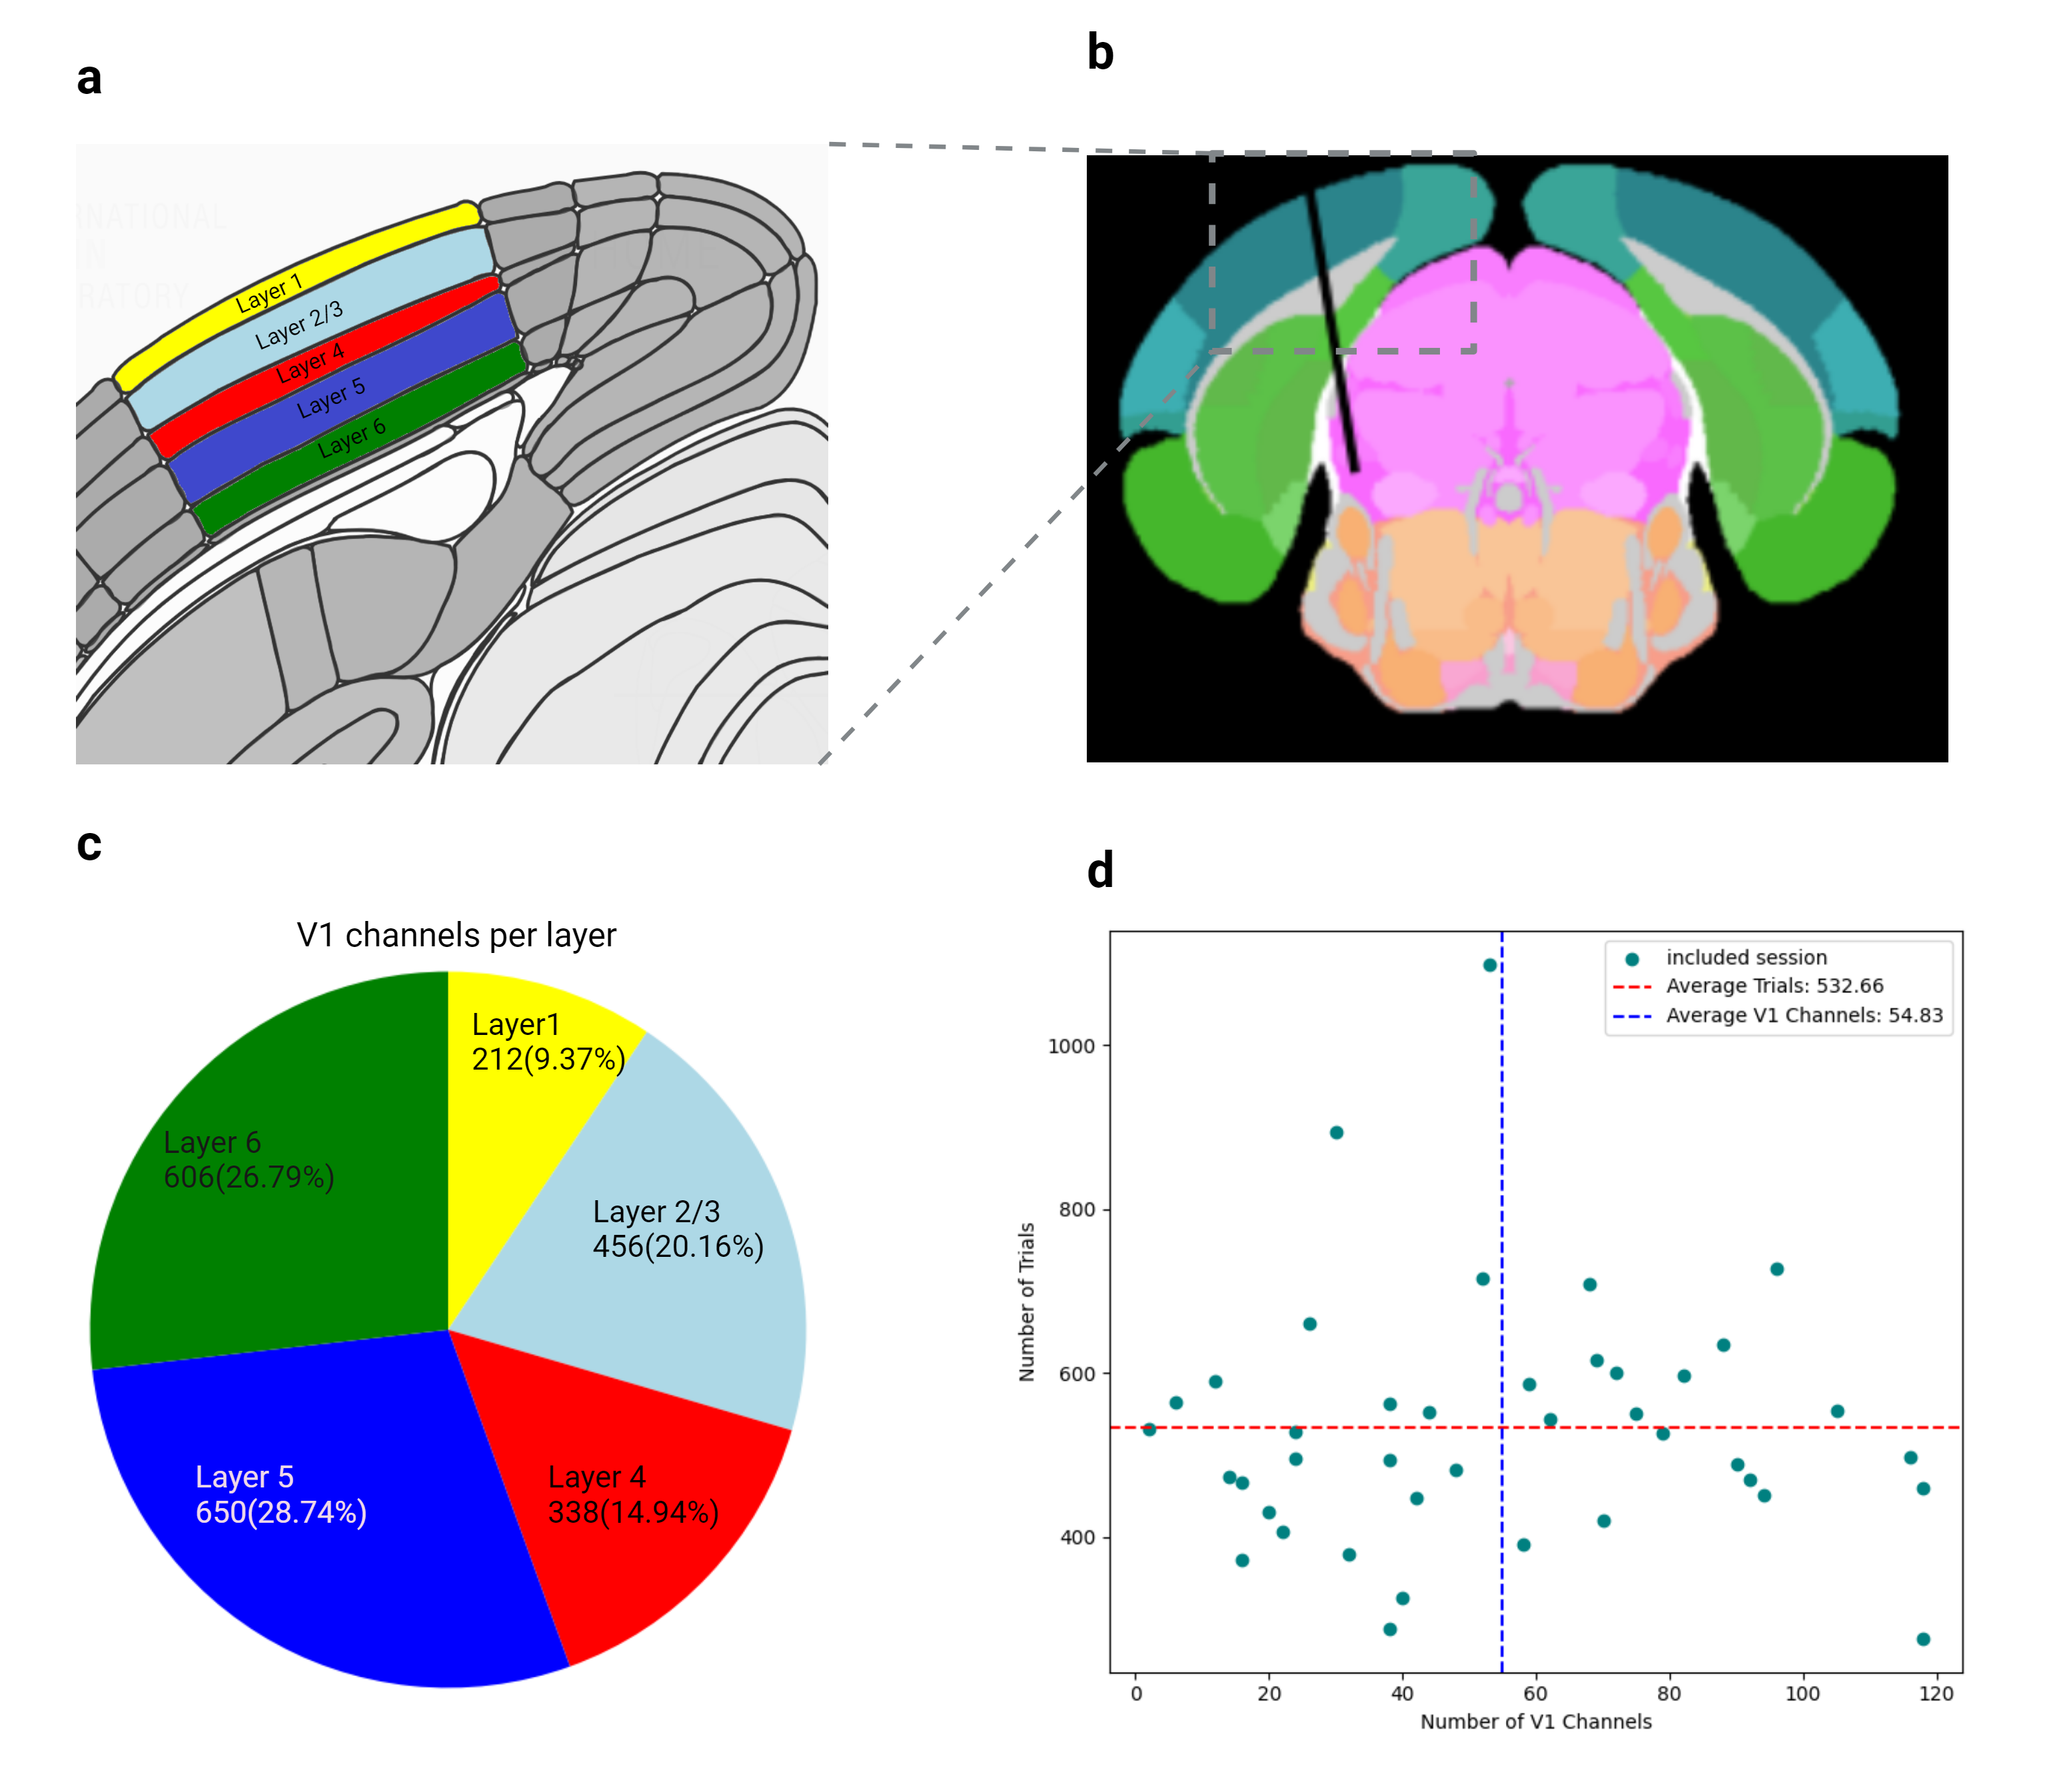
\includegraphics[width=5.97917in,height=\textheight]{images/summary.png}

}

\caption{\textbf{Figure XXX. Region of interest and recording site
locations. a)} Coronal slice of the Allen Brain Atlas, highlighting the
layers of the primary visual cortex (V1) with distinct colors: yellow
for layer 1, light blue for layers 2/3, red for layer 4, blue for layer
5, and green for layer 6. The image base is extracted from the Allen
Brain Atlas (\url{https://atlas.internationalbrainlab.org}) at an
Anterior-Posterior (AP) coordinate of -3140 µm . \textbf{b)} Coronal
slice from the Allen Brain Atlas that shows an example of a probe
insertion site in a mouse brain (subject name: NYU-12). The black line
represents the probe path, starting in V1 and ending in the midbrain
reticular nucleus (approximately). The image is taken from the IBL
online data visualization tool
(\url{https://viz.internationalbrainlab.org}). \textbf{c)} Pie chart
illustrating the proportional distribution of each V1 layer, using the
same color scheme as in panel (a). \textbf{d)} Scatter plot showing the
number of trials (range: 276-1098) and channels (range: 2-118) for the
included sessions. The mean number of channels (54.83) is indicated by a
dashed blue vertical line, and the mean number of trials (532.66) is
represented by a dashed red horizontal line.}

\end{figure}%

\subsection{\texorpdfstring{Behavioral results
}{Behavioral results }}\label{behavioral-results}

In line with previous results on whole sessions, mice performed
correctly on 80.7\% ± 5.8\% (mean ± s.d.) of the trials with reaction
time (RT) of 1.73 ± 5.7 seconds (mean ± s.d.). RT is defined as the time
interval between stimulus onset and when wheel rotation reach threshold
of 35° ; and performance is computed as a percent of correct trials over
total number of trials. As illustrated in (fig X a;b), Performance
improved and reaction times decreased on trials with higher stimulus
contrast. In 0\% contrast trials, where mice had to rely only on their
expectation and prior experience, they made correct choices in 57\% ±
8\% (mean ± s.d.).

\begin{figure}[H]

{\centering 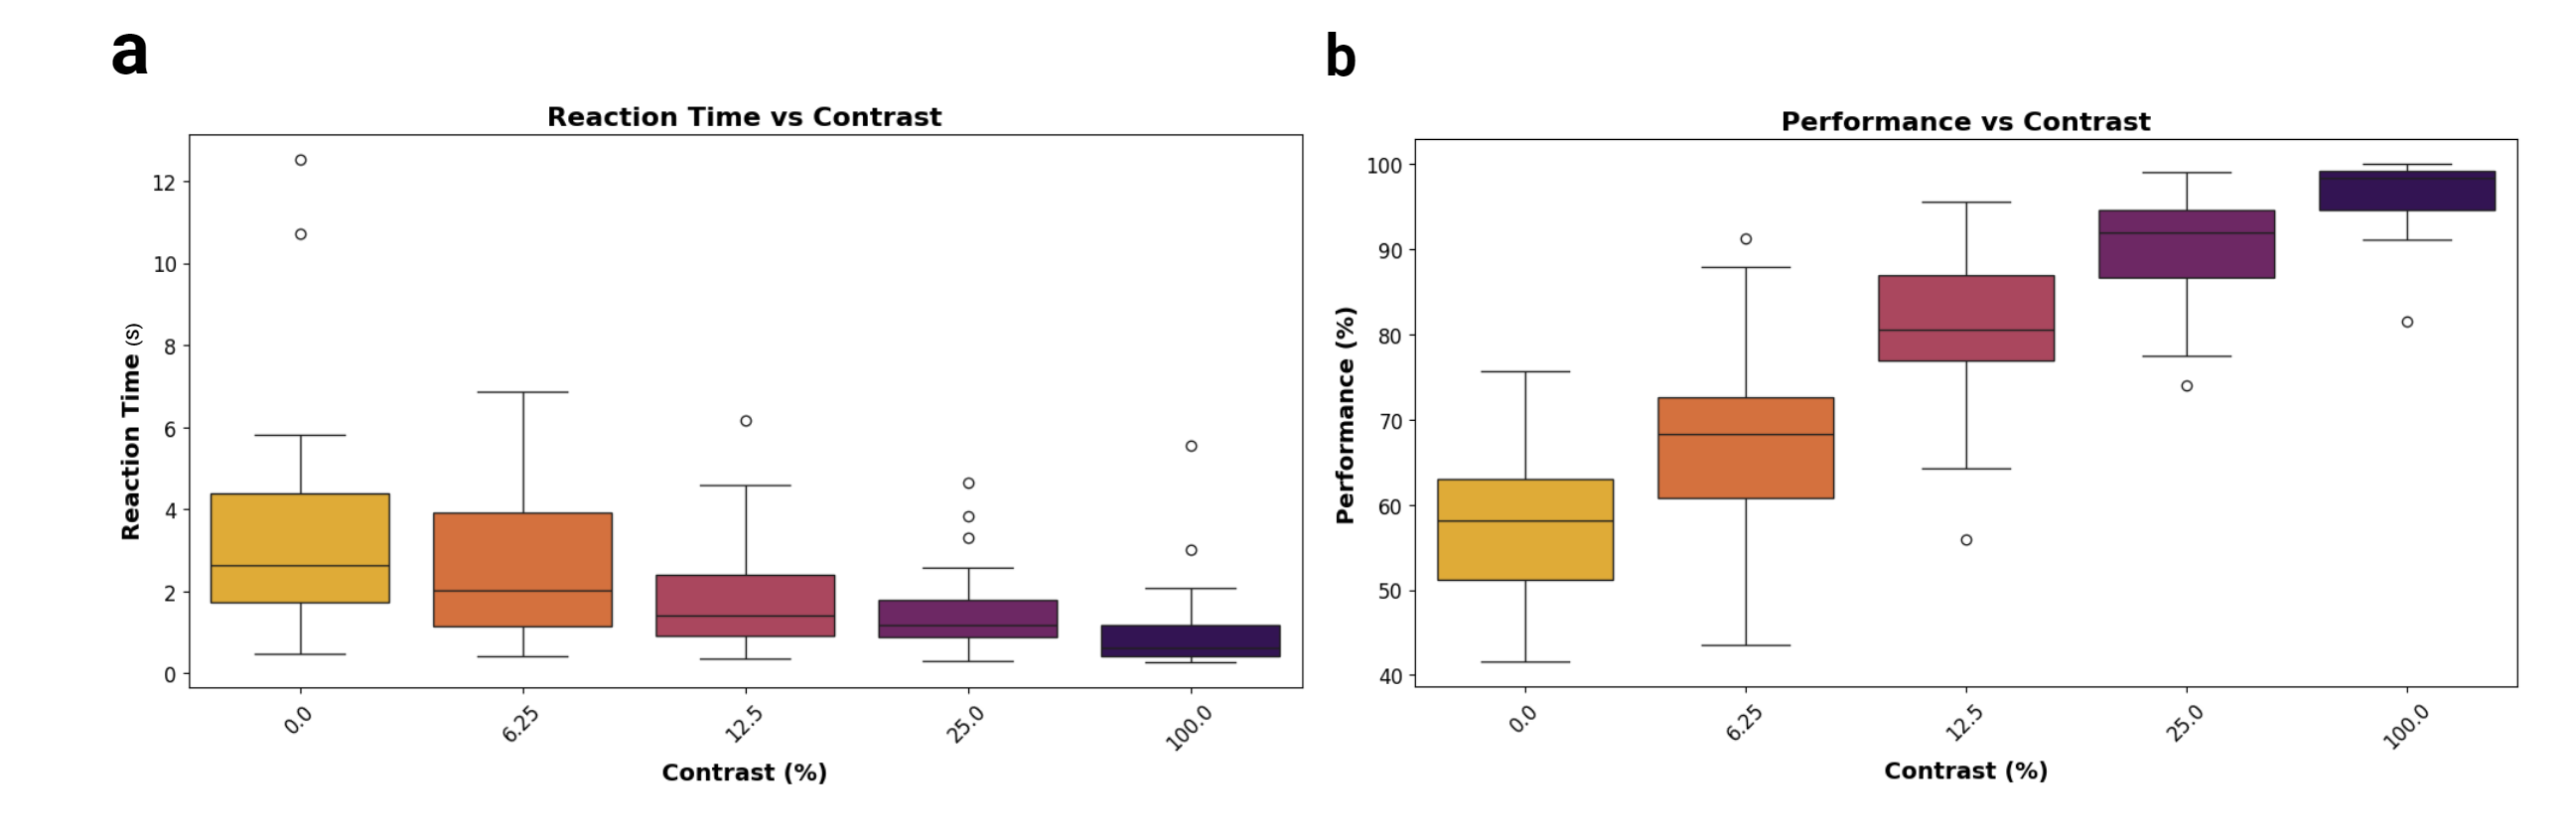
\includegraphics{images/behavioral.png}

}

\caption{\textbf{Figure XXX. Behavior results.} \textbf{a)} illustration
of reaction time for different stimulus contrast level using boxplot.
\textbf{b)} Illustration of performance (as a percent of correct trials
over total number of trials) for each contrast levels using boxplots. }

\end{figure}%

\subsection{Inter trial phase coherence
(ITC)}\label{inter-trial-phase-coherence-itc-1}

The ITC analysis indicated significant phase alignment in the
low-frequency range (2-8 Hz) within the {[}0, 0.5{]} second interval
following the stimulus (see Fig. X a). To ensure that these findings
were not due to chance and to correct for multiple comparisons, we
applied the MNE one-sample cluster permutation test (refer to the
Statistical Analysis section of the Methods for more details ). The
significant clusters, marked by the black line in Fig. X a , demonstrate
that the low-frequency ITC during the 0-0.5 second period was
statistically meaningful, with a p-value of 0.001. Additionally, as
illustrated in Fig. X c, there were no significant differences in ITC
across the V1 layers in the low-frequency range.

To assess whether the observed ITC levels were influenced by the
stimulus, ITC average levels were compared for each level of stimulus
contrast. The average ITC was computed for the low-frequency range (2-8
Hz) and within the 0-0.5 second time window post-stimulus. As
illustrated in Fig. X b, an increase in stimulus contrast generally
resulted in a higher mean ITC. Interestingly, the only group of trials
that did not support this trend was trials without stimulus
(i.e.~contrast 0\%), which will be discussed in the next section.

To statistically evaluate whether the mean ITC was significantly
affected by contrast levels, further analysis was undertaken. Given that
the Shapiro-Wilk normality test did not confirm normality in the data
distribution, the Friedman test, a non-parametric alternative to
repeated measures ANOVA, was employed. The results of the Friedman test
indicated a highly significant effect of contrast level on ITC mean,
with a test statistic of 77.98 and a p-value of
4.66*10\textsuperscript{-16}, indicating that variations in ITC across
different contrast levels were unlikely to have occurred by chance. Due
to the significant effect of contrast level on ITC mean identified by
the Friedman test, a post-hoc Nemenyi test was performed to determine
which specific contrast levels contributed to the observed differences.
The Nemenyi test was chosen as it is appropriate for pairwise
comparisons following a Friedman test. The post-hoc analysis results are
presented in fig \ul{X d,} with p-values indicating the significance of
differences between each pair of contrast levels.

\begin{figure}[H]

{\centering 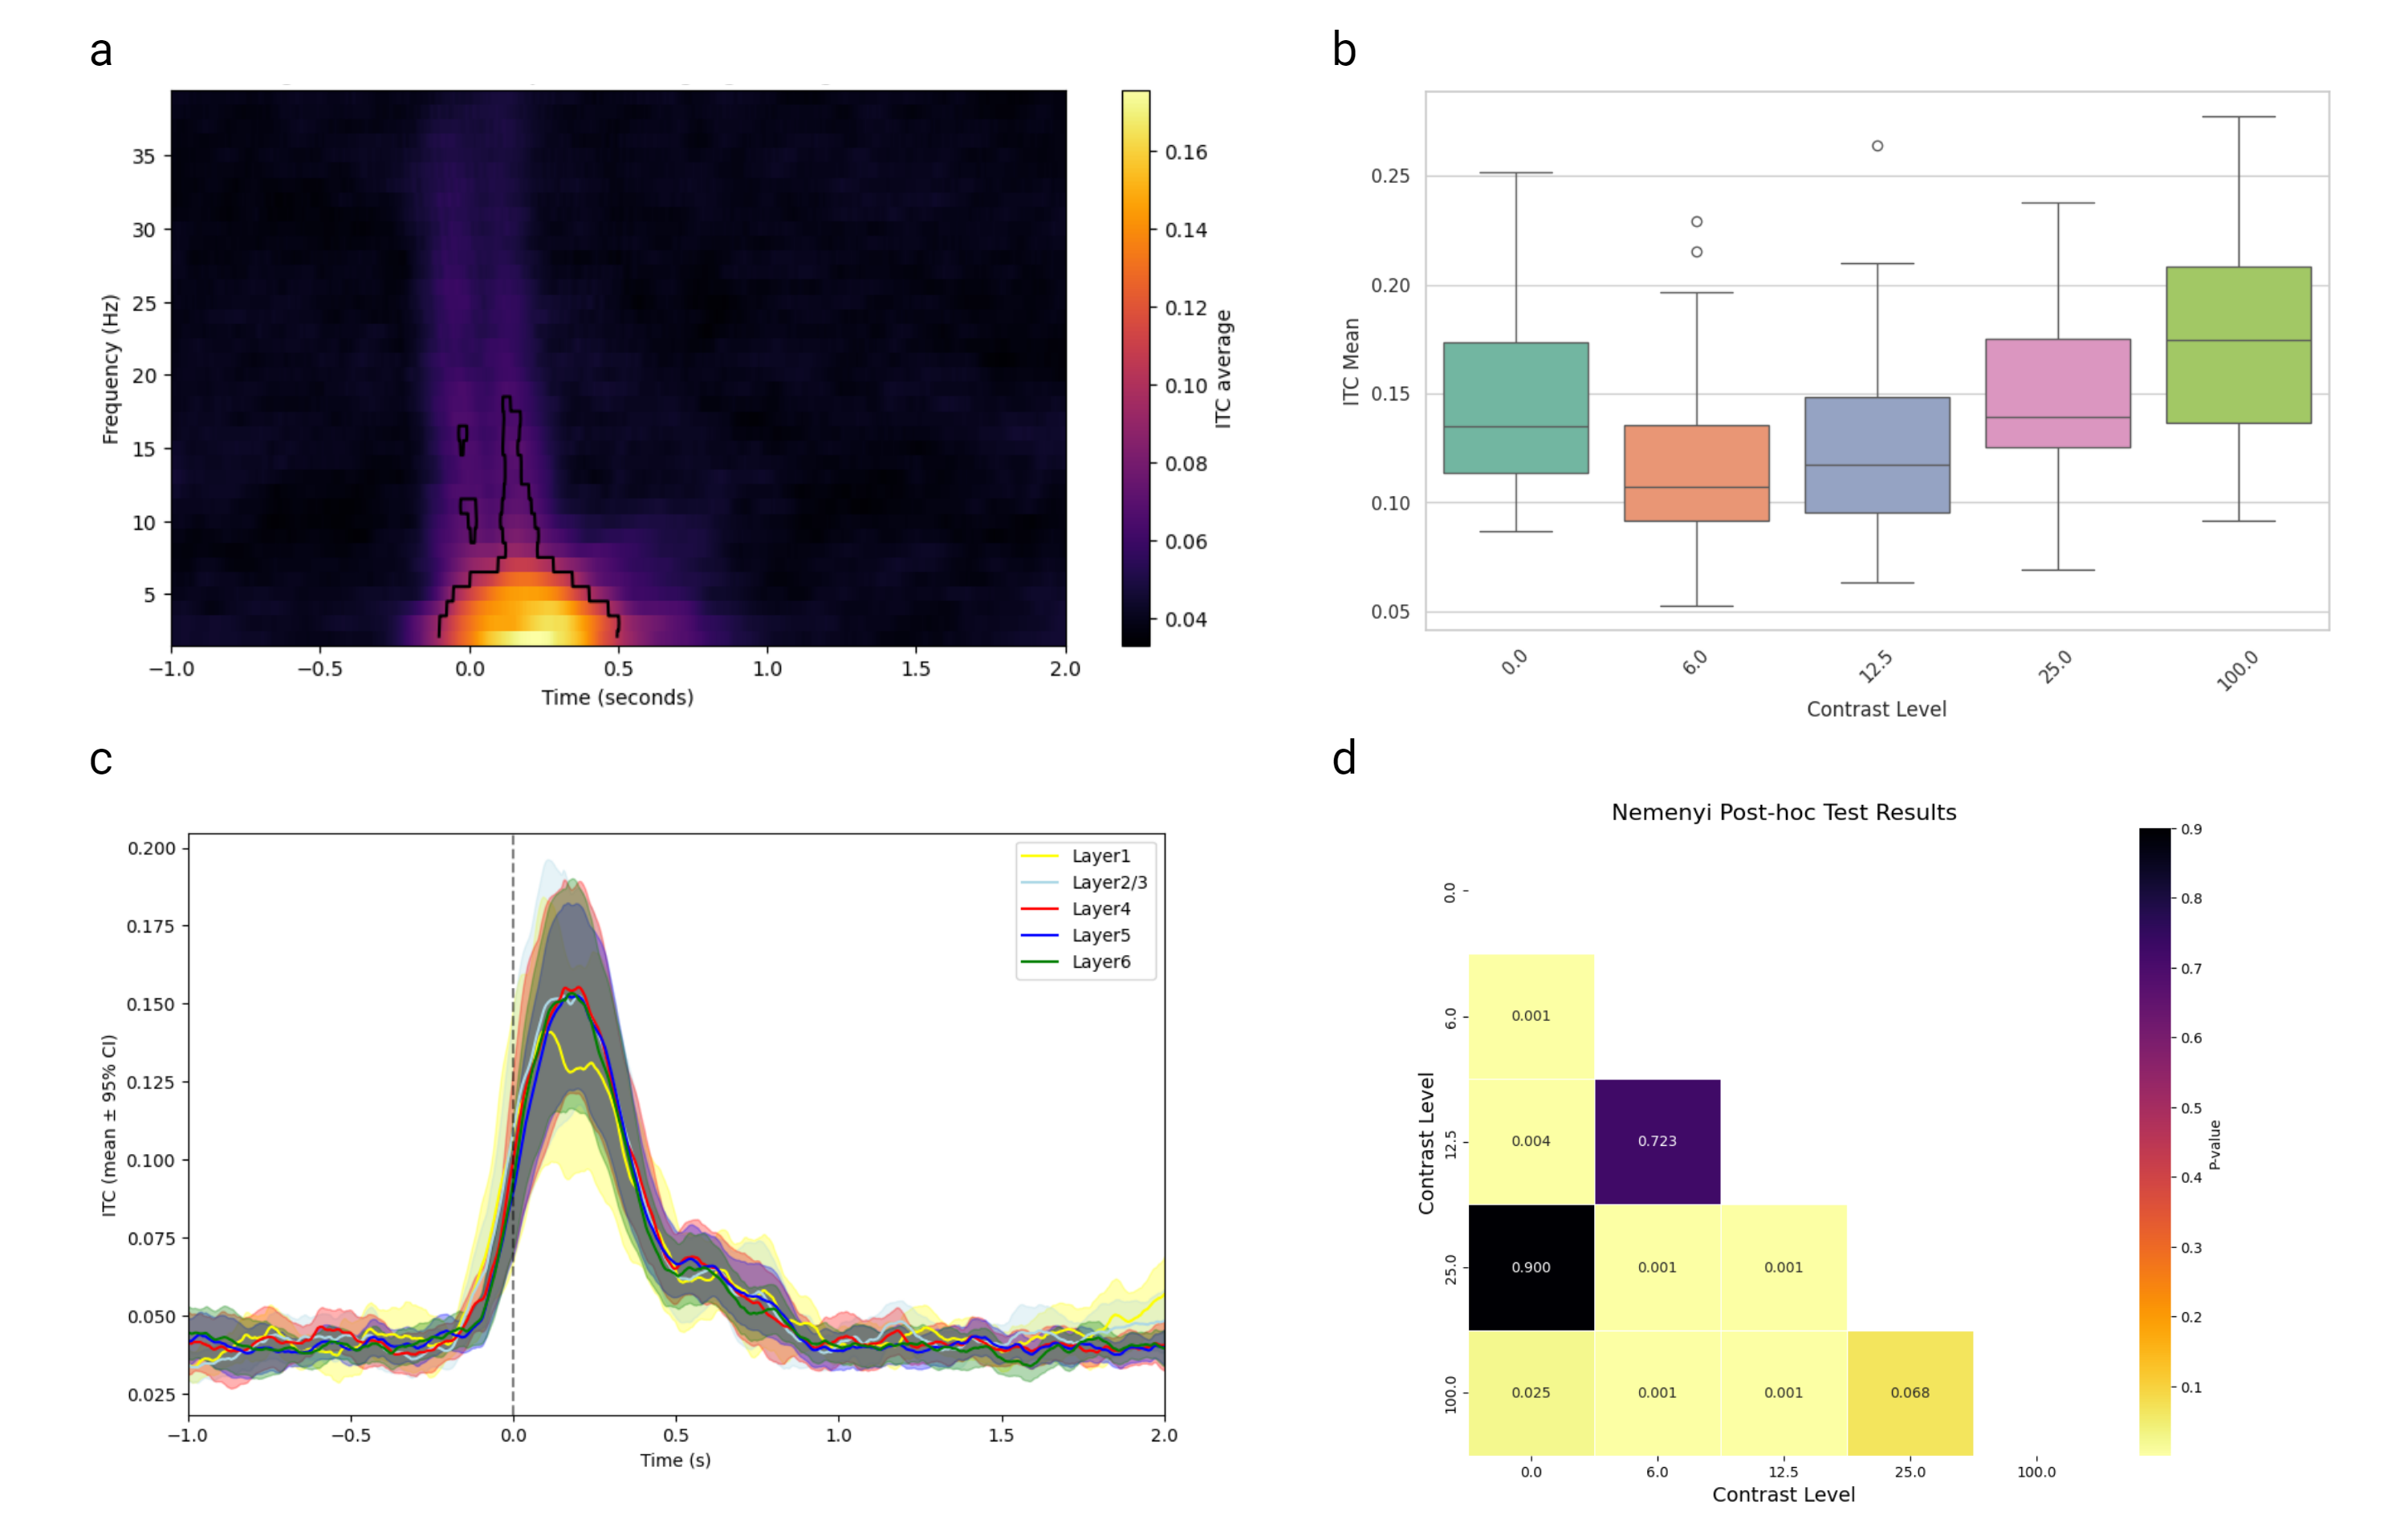
\includegraphics{images/ITC.png}

}

\caption{\textbf{Figure XXX. Inter trial phase coherence (ITC).}
\textbf{a)} ITC average across all subjects and cortical layers relative
to stimulus onset. Significant clusters (p = 0.001) are indicated by
black lines, as determined by the MNE one-sample cluster permutation
test.\textbf{b)} Comparison of ITC averages across different stimulus
contrast levels using a box plot. The ITC average was computed for the
2-8 Hz frequency range within the 0-0.5 second time window
post-stimulus, aggregated across all subjects and layers. \textbf{c)}
Low-frequency ITC averages for each V1 layer relative to stimulus onset.
The layer-specific averages are depicted with solid lines, and their
95\% confidence intervals are shaded around the lines in distinct
colors: yellow for layer 1, light blue for layers 2/3, red for layer 4,
blue for layer 5, and green for layer 6. \textbf{d)} Nemenyi post-hoc
test p-value results for each pair of contrast levels. Lower p-values
indicate significant differences between the ITC average distributions
for each pair, represented by a heatmap ranging from yellow (low
p-values) to black (high p-values). }

\end{figure}%

\subsection{Time frequency analysis
results}\label{time-frequency-analysis-results}

Although there was substantial variability across subjects, the
time-frequency analysis of V1 revealed two notable oscillations in
relation to the visual stimulus: first, an increase in high-frequency
power within the gamma band range (20--40 Hz), and second, a concurrent
decrease in lower-frequency power within the 2--7 Hz range. The gamma
increase was more transient, while the lower frequency inhibition
persisted for a longer duration (see Figure X). As shown in Figure Xa,b,
the observed frequency band changes exhibited a similar pattern across
the different layers of V1. Statistical tests were not applied to
quantitatively evaluate the layer-specificity of these effects, as the
variability in the number of channels across layers and subjects did not
allow for such an analysis.

The averaged power of each frequency band over the first 1 second after
the stimulus was compared for trials with different contrast levels. The
Friedman test revealed a statistically significant effect of contrast
level on power modulation in both the low-frequency band (test
statistic: 20.54, p-value: 0.00039) and the gamma band (test statistic:
18.88, p-value: 0.00083), indicating that power in these bands was
significantly influenced by the stimulus contrast. However, as you can
see in Figure Xa,b, the frequency band average power across different
contrast levels is not quite observable. Additionally, the post-hoc test
results shown in Figure Xc,d indicate that the comparisons were mainly
significant only in comparison to the 100\% contrast condition.

This not readily observable difference is believed to be mainly due to
inter-subject variability, with some subjects showing significant
contrast-related modulations, while others do not. In general,
especially in sessions with high effects of contrast on power bands,
higher contrast stimuli involved greater increases in gamma and
decreases in theta band power.

\begin{figure}[H]

{\centering 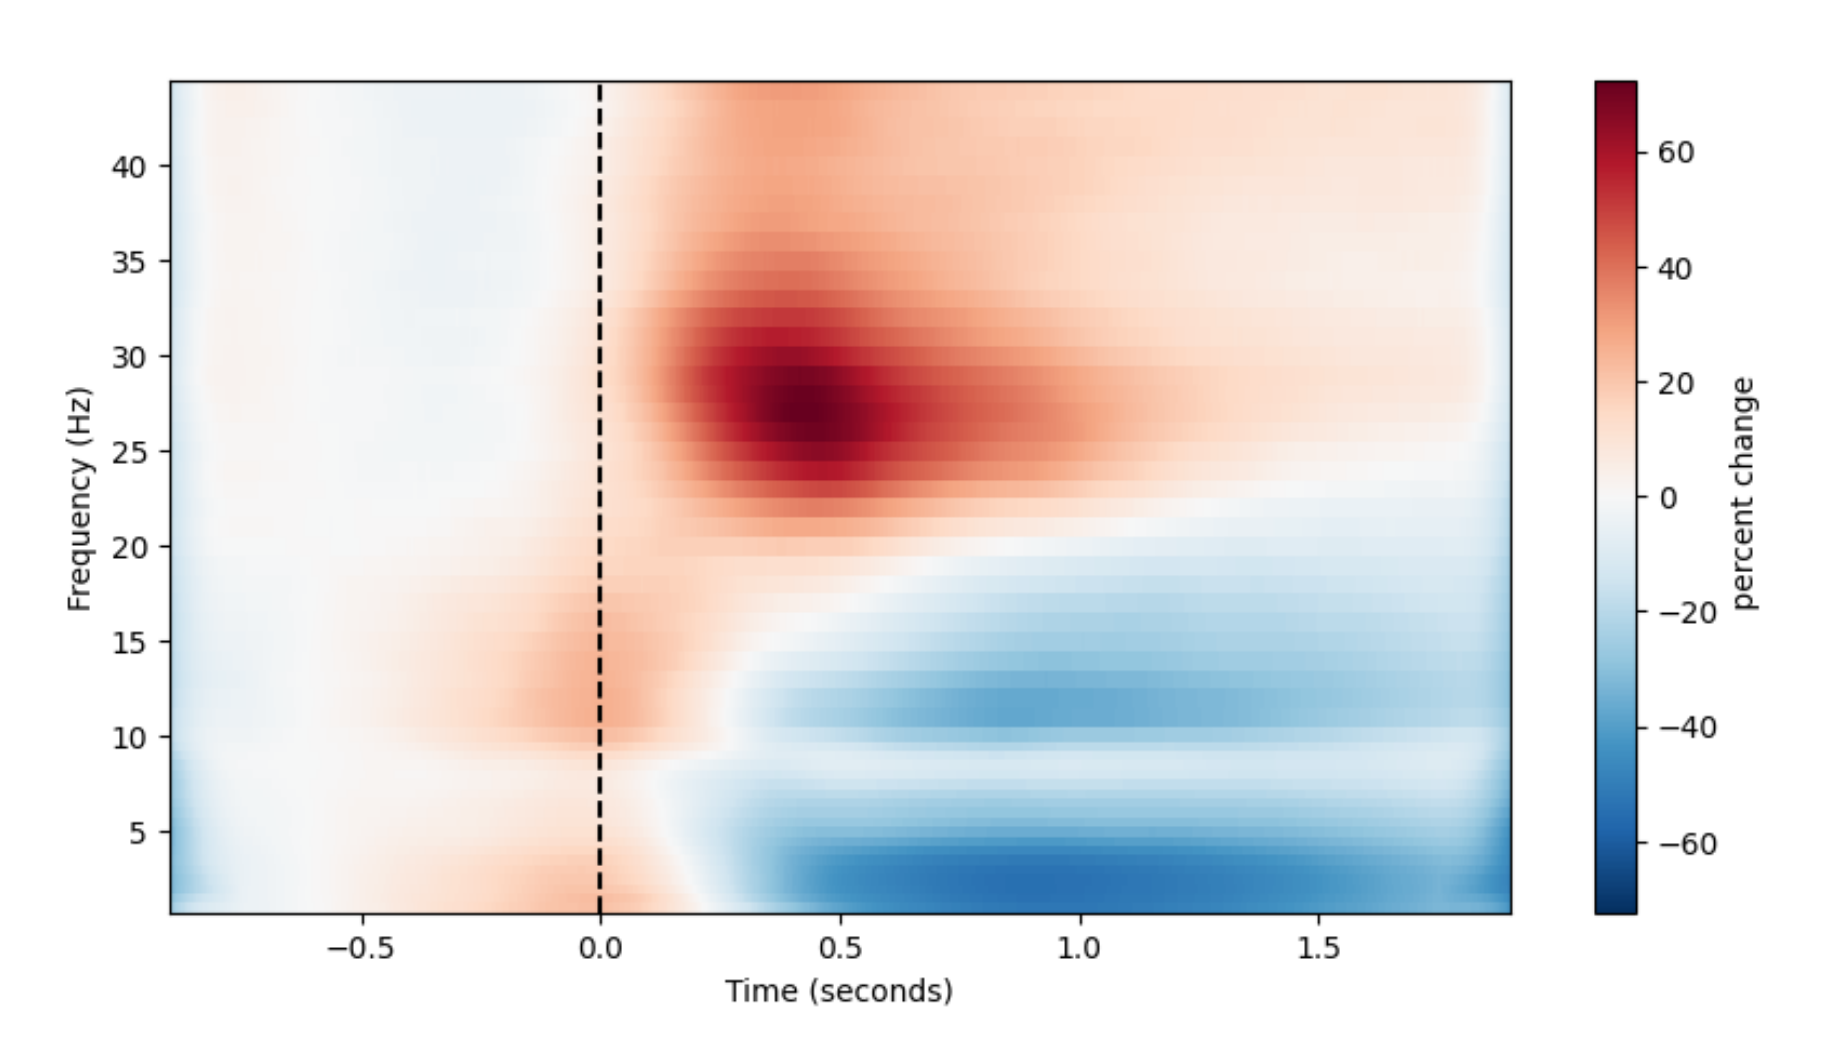
\includegraphics[width=7.30208in,height=\textheight]{images/TF.png}

}

\caption{\textbf{Average time frequency representation.} Time-frequency
is averaged over all channels in the primary visual cortex, computed
using the multitaper method. The data is baseline-corrected using the
-0.7 to -0.5 s pre-stimulus interval, with time relative to stimulus
onset (marked by dashed black vertical line). Power is shown in percent
units with a blue-to-warm colormap.}

\end{figure}%%
\begin{figure}[H]

{\centering 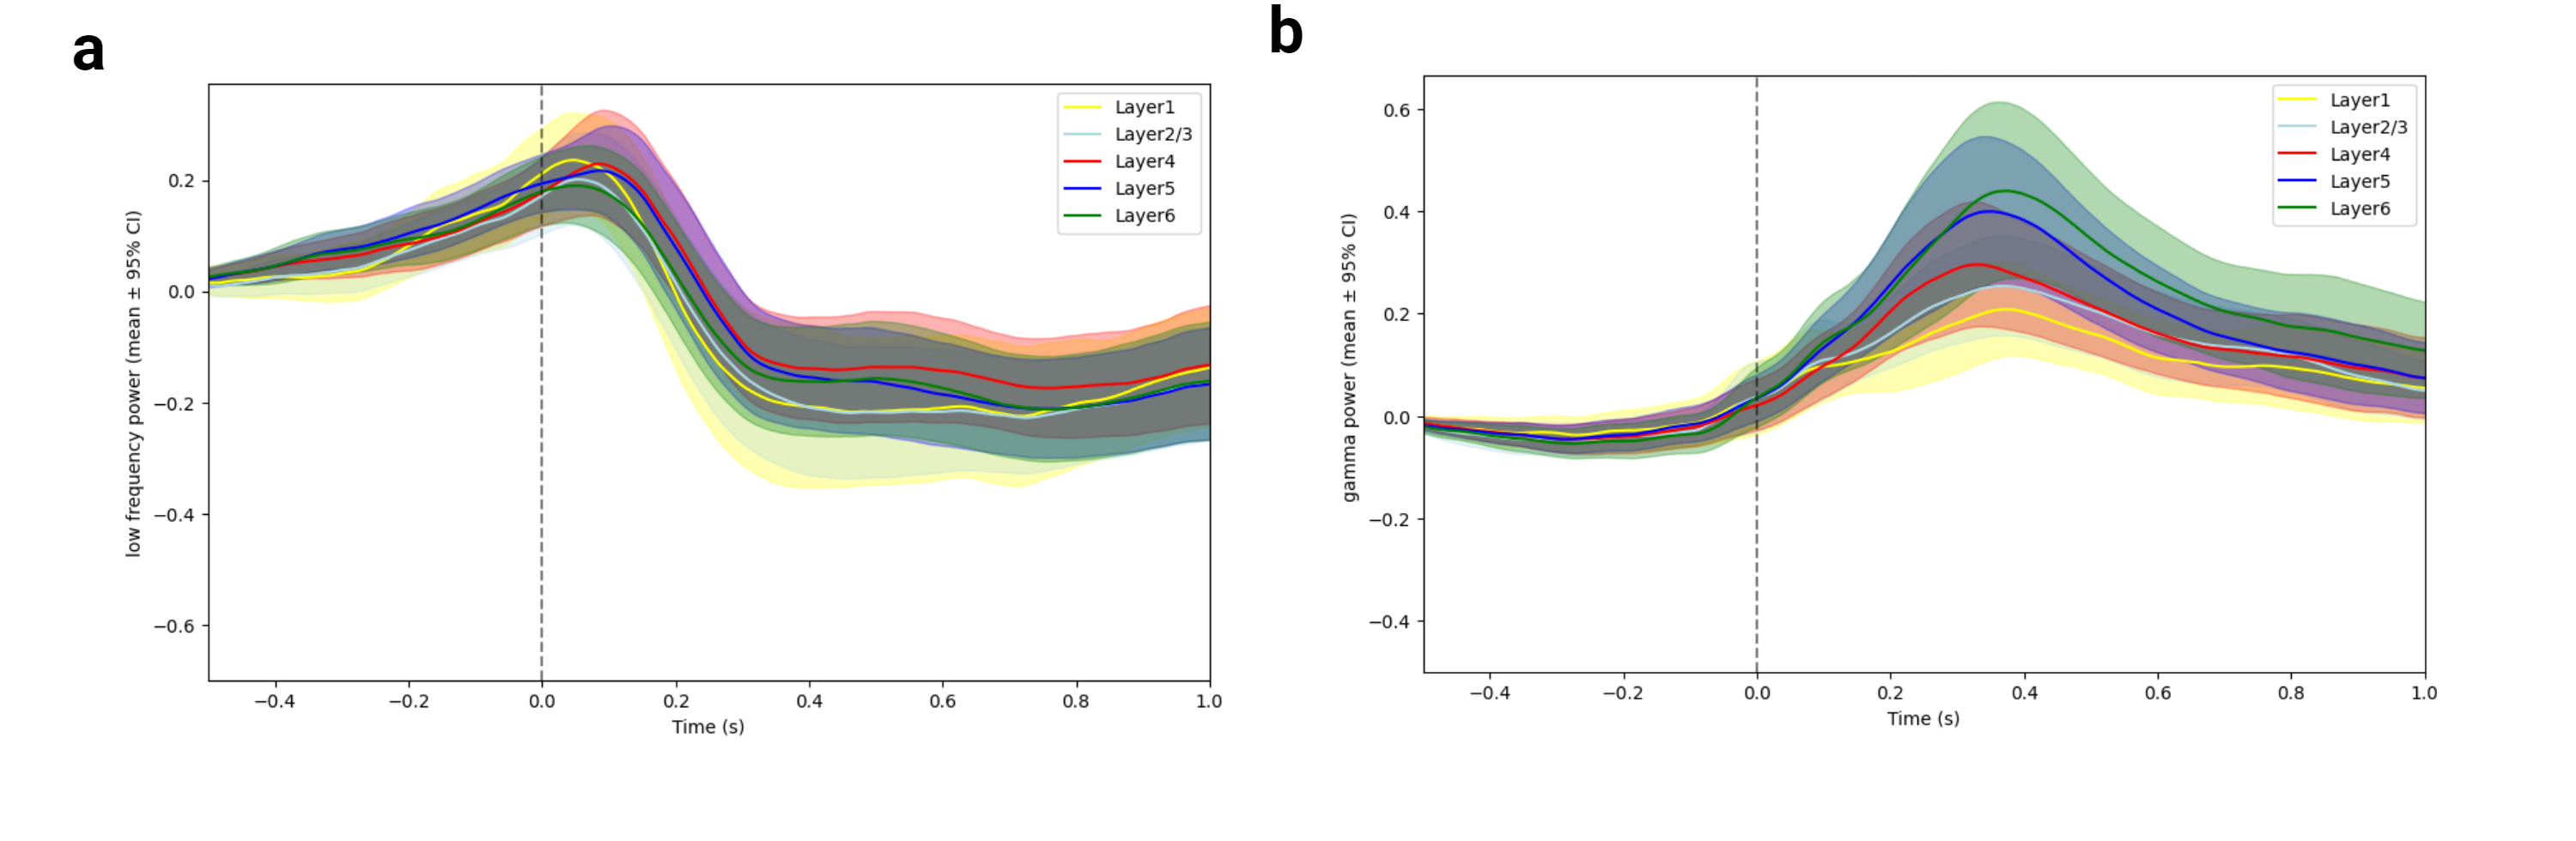
\includegraphics{images/layer_power.png}

}

\caption{\textbf{Average frequency band power across time for all layers
of V1}. \textbf{a)} low frequency (2-7 Hz) average power for each V1
layer relative to stimulus onset (marked by dashed black vertical line).
The layer-specific averages are depicted with solid lines, and their
95\% confidence intervals are shaded around the lines in distinct
colors: yellow for layer 1, light blue for layers 2/3, red for layer 4,
blue for layer 5, and green for layer 6. \textbf{b)} similar to panel
(a) but for higher frequency band (20-40 Hz)}

\end{figure}%%
\begin{figure}[H]

{\centering 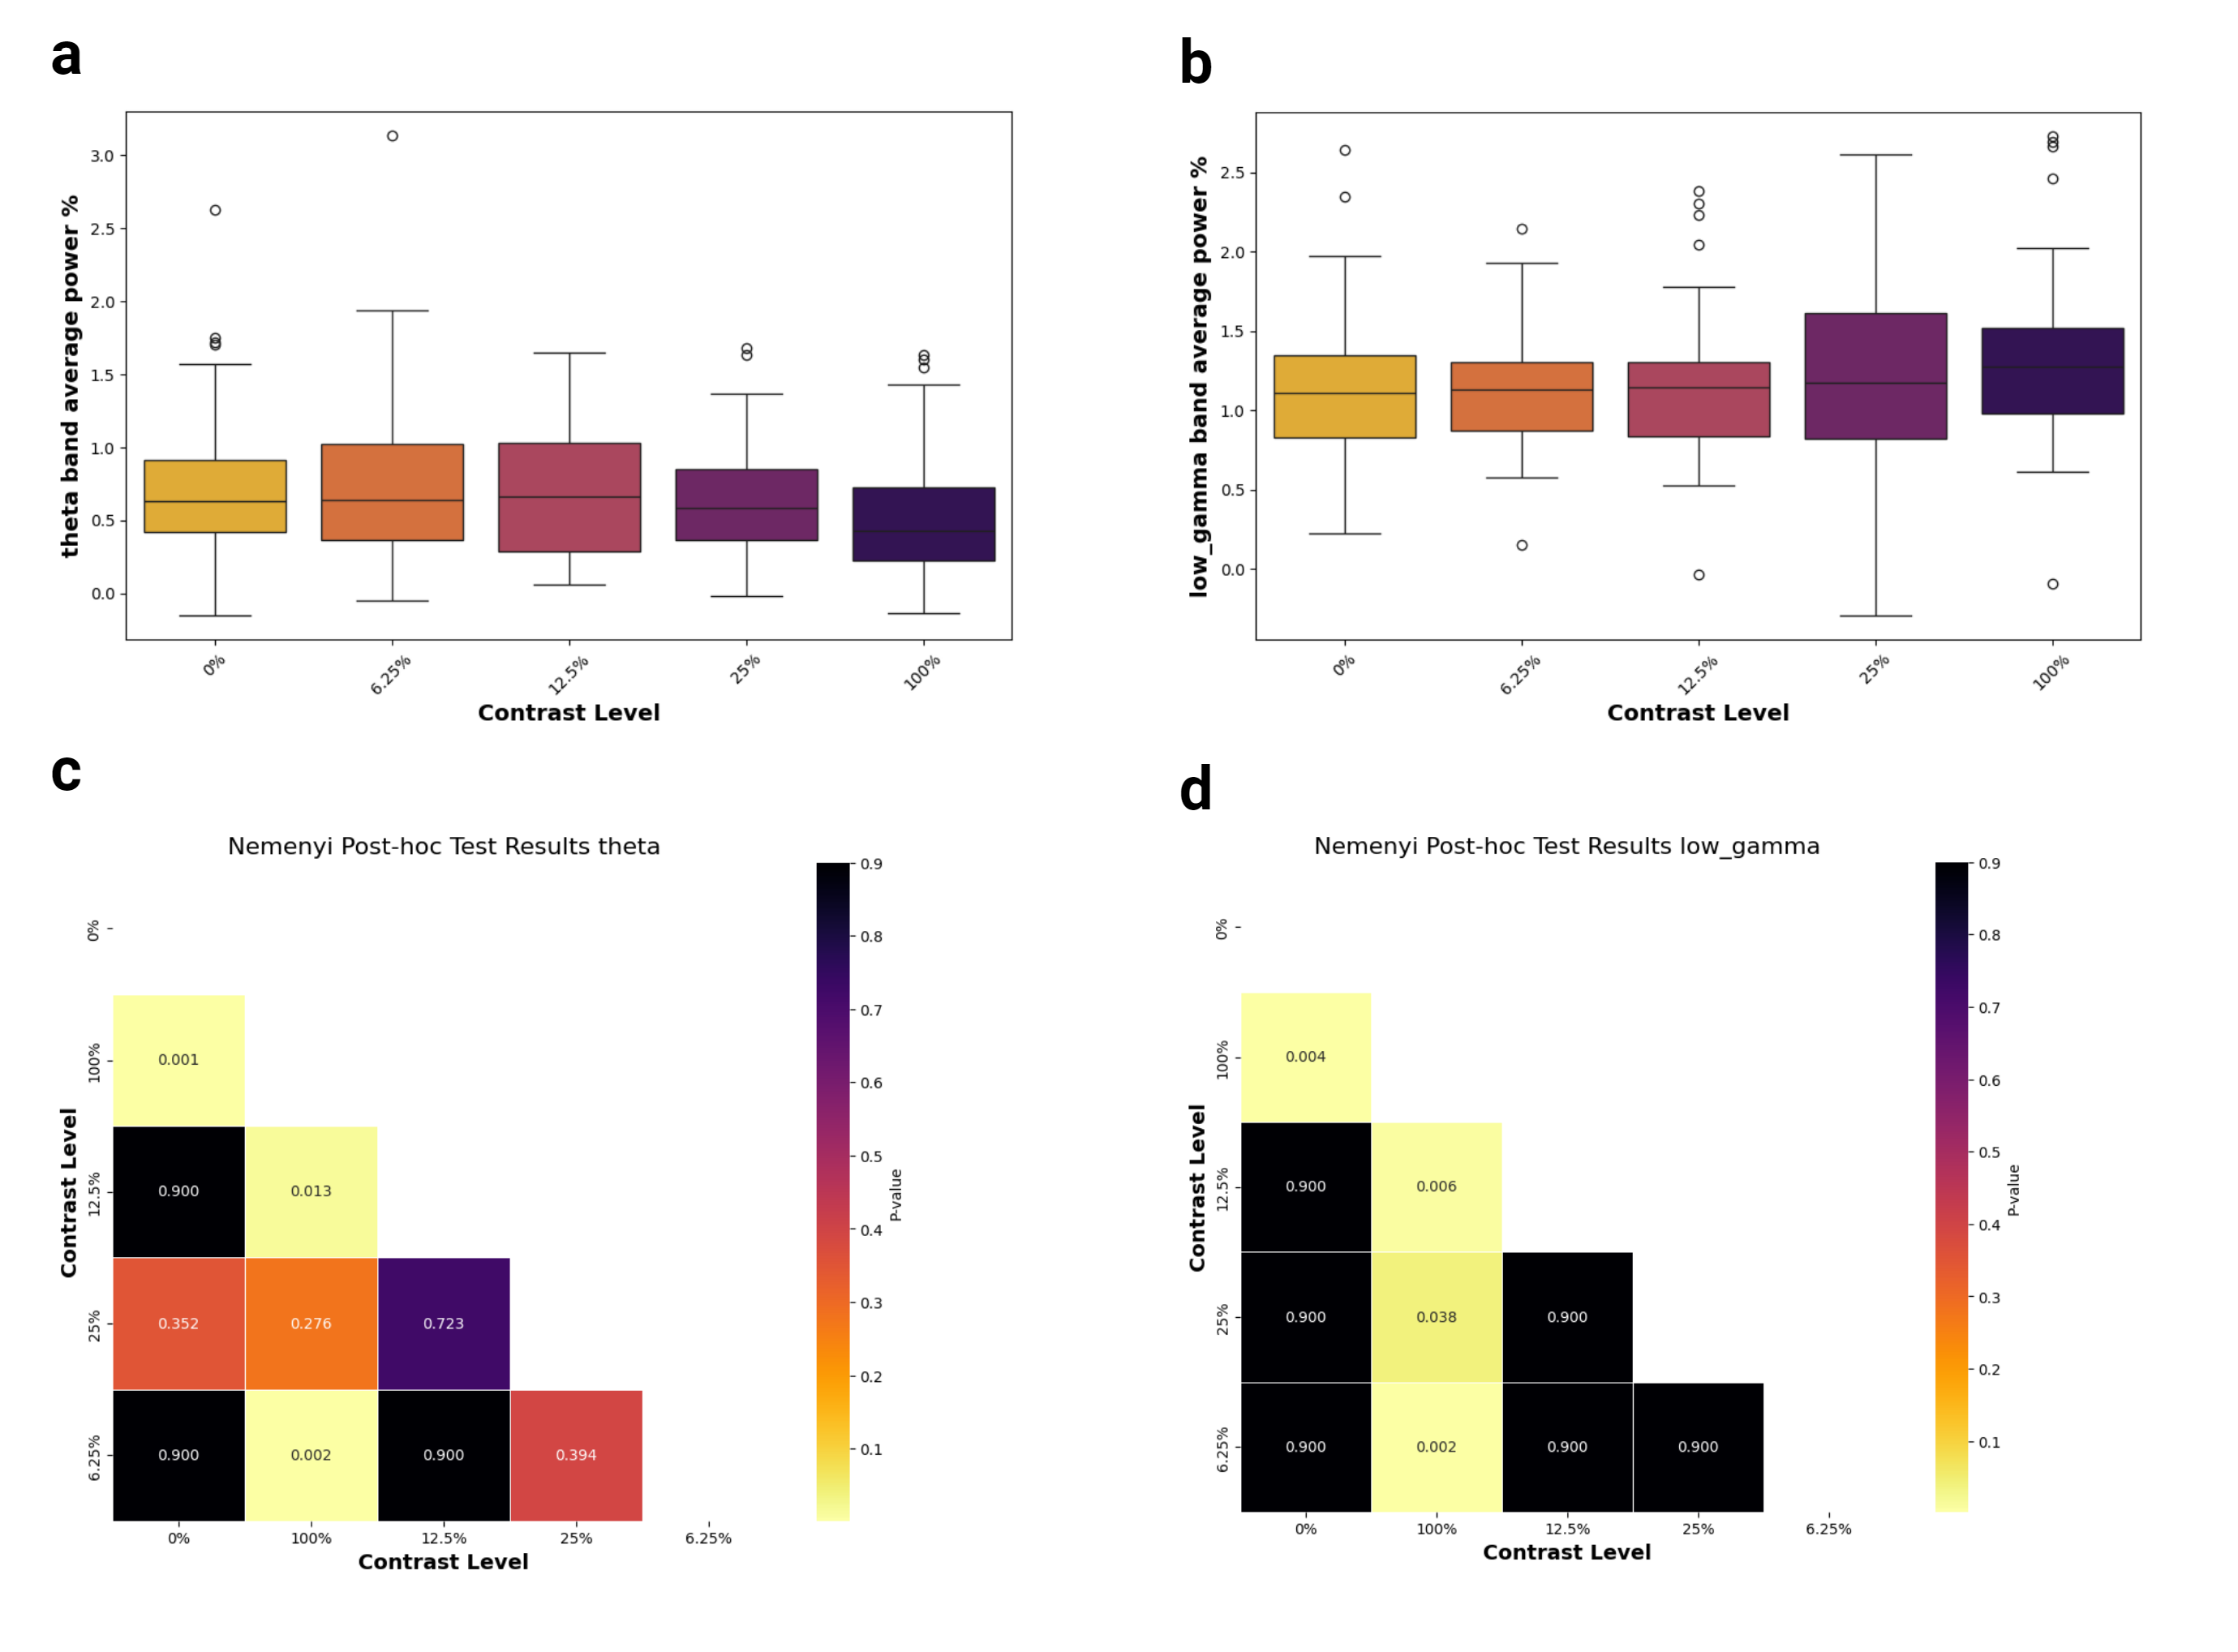
\includegraphics[width=7.05208in,height=\textheight]{images/contrast_power.png}

}

\caption{Affects of stimulus contrast on low and high frequency average
power. \textbf{a)} The box plots represents the distribution of
low-frequency (2-7 Hz) average power across different contrast
levels.The power is averaged over the first 1 second after stimulus
across all channels of each subject (N= 41). The central line in each
box indicates the median power average value, while the box edges
represent the inter-quartile range (IQR) and whiskers extend to 1.5
times the IQR. \textbf{B)} similar to panel (b) but for high frequency
range (20-40 hz). \textbf{C)} Nemenyi post-hoc test p-value results
comparing low frequency average power for pairwise contrasts levels.
Lower p-values indicate significant differences between the low
frequency average power distributions for each pair, represented by a
heatmap ranging from yellow (low p-values) to black (high p-values).
\textbf{d)} similar to panel (c) but for high frequency (20-40 Hz)
average power}

\end{figure}%

\subsection{Phase amplitude coupling
(PAC)}\label{phase-amplitude-coupling-pac}

Phase-amplitude coupling (PAC) analysis revealed that the phase of
low-frequency oscillations (2-7 Hz) modulates the amplitude of
high-frequency oscillations (25-80 Hz). In Figure X, an example from a
single channel illustrates how the amplitude of high-frequency
oscillations changes depending on the phase of low-frequency
oscillations during the period after the stimulus. This example visually
demonstrates the coupling effect; however, it is important to note that
this figure serves solely as an illustration of the amplitude modulation
by phase, and no specific coupling method (e.g., Gaussian copula) was
applied to quantify this effect.

\begin{figure}[H]

{\centering 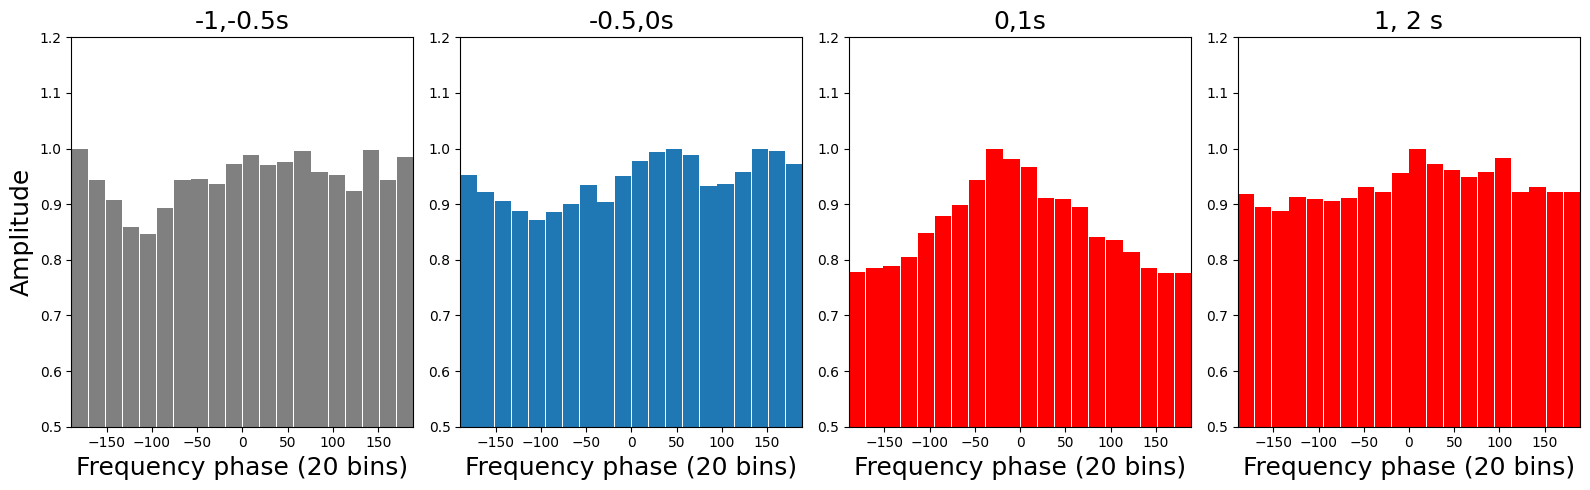
\includegraphics{images/bin_amplitude.png}

}

\caption{\textbf{Binned Amplitude by Phase for a channel in V1}. This
figure illustrates the binned amplitude of high-frequency oscillations
(25-80 Hz) as a function of the phase of low-frequency oscillations (2-7
HZ) for four time windows. From left to right : (-1, -0.5), (-0.5, 0),
(0, 1), and (1, 2) with time in seconds relative to the stimulus onset.
The data were binned into 20 equal-sized phase bins, and the amplitude
was averaged within each bin. The non-uniform distribution of amplitudes
indicate high possibility of coupling. As you can see, the time period
one second after stimulus (0, 1s) shows observable non-uniform
distribution of amplitudes with the highest value for phase zero. This
plot is intended to illustrate the relationship between phase and
amplitude without applying any coupling quantification. The plot is made
using Tensorpac python module (Combrisson et al. 2020).}

\end{figure}%

Comparing PAC values for the time periods before and after the stimulus
revealed a significant increase in PAC values following the stimulus.
This difference was confirmed by a repeated measures ANOVA, which
resulted in F = 5.503, p = 0.0242. The distribution of average PAC
values before the stimulus was centered slightly towards negative values
(mean: -0.05) and exhibited large tails in both positive and negative
directions (standard deviation: 0.05). In contrast, the distribution of
PAC values after the stimulus was centered on positive values (mean:
0.02) with narrower tails (standard deviation: 0.01) (see Figure Xa).

In addition, we found that this difference between PAC values were more
pronounced in layer five and six (see Figure Xb). As illustrated in
Figure X, these two V1 layers were the only layers with F values higher
than F-critical (approximately 4). However , similar to Time frequency
analysis, no further statistical tests

were applied to quantitatively evaluate the layer-specificity due to the
variability in the number of channels across layers.

\begin{figure}[H]

{\centering 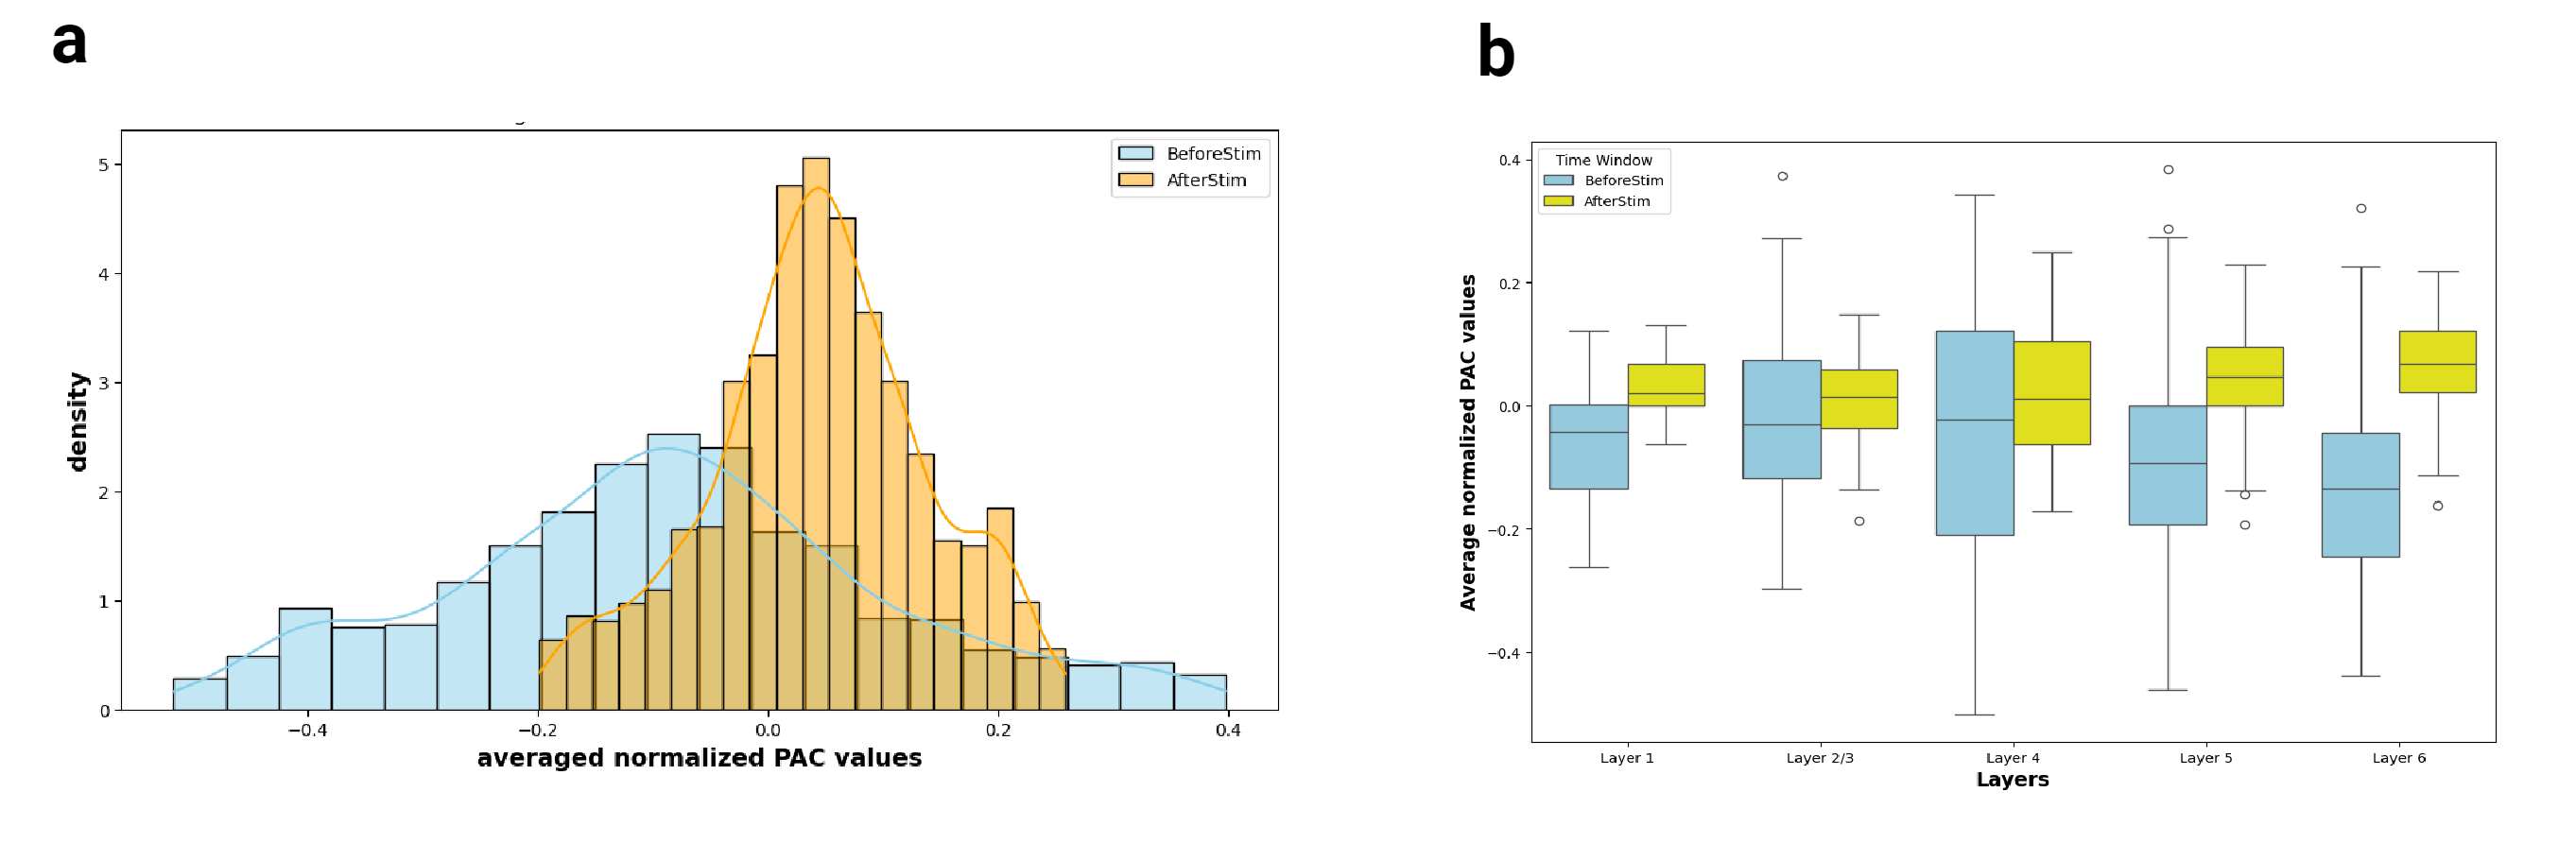
\includegraphics{images/pac_beforeVSafter.png}

}

\caption{Phase Amplitude Coupling (PAC) values before and after
stimulus. a) Histogram distribution of averaged normalized PAC values
for frequency of phase (2-7 HZ) and frequency for amplitude of (25-80
HZ). The distribution is across all V1 channels (N = 2,262) and for two
time period: after stimulus (0-1 s) with color yellow and before
stimulus (-0.5, 0 s) with color light blue. The histograms are computed
with 20 bins, and a kernel density estimate (KDE) is overlaid with solid
line. B) Boxplot illustration of before (yellow) and after (light blue)
stimulus PAC values for each layer of V1, with number of channels per
layer : layer1 = 212, layer 2/3: 338, layer 4 = 650, layer 5 = 650,
layer 6 = 606. As you can see the difference is significant mainly in
layer 5 and 6.}

\end{figure}%

\section{Discussion}\label{discussion}

According to predictive coding, High-frequency feedforward (FF) and
low-frequency feedback (FB) oscillations contribute to the hierarchical
processing of sensory stimuli by generating predictions and attaching
behavioral context to the sensory world(Aggarwal et al. 2022). Yet, the
role of these oscillations in shaping perception remains poorly
understood, particularly in mice. The International Brain Laboratory
(IBL) open-access datasets, with their sophisticated experimental
paradigms and large-scale neural recordings, provide an unprecedented
opportunity to study the principles of predictive coding in mice. In
this project, we analyzed the IBL local field potential data from the
primary visual cortex (V1) as a first step towards utilizing this
dataset to understand the principles of predictive coding and
communication through oscillation.

\subsection{Main results in respect to previous
studies}\label{main-results-in-respect-to-previous-studies}

The inter trial phase coherence (ITC) analysis revealed a significant
theta (2-5 Hz) phase coherence within the first 500 ms after visual
stimulation. This frequency and temporal range of observed phase
coherency is totally consistent and similar to previous study in mice
(Aggarwal et al. 2022). The time frequency (TF) analysis showed an
increase in low gamma (25-40 HZ) power with concurrent decrease of theta
power after visual stimulation. Consistent with presumed FF-FB roles of
these high and low frequency band power we found shorter and transient
peak in low gamma with longer lasting theta decrease. In addition, these
results add another evidence to the previous line of thought Senzai,
Fernandez-Ruiz, and Buzsáki (2019) that suggests the functional
properties of theta oscillation in mice are analogous to primate alpha
oscillations (7-15 HZ) including an anti correlation with local firing
rate and decreased power upon visual stimulation.

By statistically analyzing the effects of stimulus contrast on ITC and
TF results, we further confirmed that the observed pattern is
significantly dependent on a characteristic of the visual stimuli. One
interesting observation was that in trials with no stimuli, the theta
dynamics in both ITC and TF did not follow the typical trend with
respect to stimulus contrast. For example, in analyzing theta phase
coherency with respect to stimulus contrast, the common trend is a
decrease in coherency as contrast decreases. Yet, the 0 contrast trials
surprisingly showed higher coherency, even slightly close to the full
contrast group. Considering theta dynamics as a signature of feedback
communication, we believe this observation could possibly indicate the
presence of two different FB signals. For instance, the theta ITC for
zero contrast could be related to an expectation FB signal because the
mouse has heard the go cue tone, while the theta ITC when there is a
stimulus could be an FB signal from higher-order areas related to the
complex features of the stimuli. As the mouse cannot see the
low-contrast stimuli well, this FB signal is lower, leading to less
theta ITC. This line of reasoning is only valid if we accept that the
theta ITC/TF pattern in no-stimulus trials is neither related to noise
nor a disproof of the effects of stimulus contrast on the observed
ITC/TF.

The phase amplitude coupling (PAC) analysis showed significant theta-low
gamma coupling after visual stimulation. This finding aligns with a
previous study in mice (Aggarwal et al. 2022) and is analogous to
alpha-gamma coupling observed in primates during sensory processing
(Spaak et al. 2012). Although this result adds important value to this
line of evidence, further analysis is needed to determine the degree to
which we can relate this PAC to task features. Similar to our previous
investigations of ITC and TF, we can start by analyzing how the contrast
of stimuli affects PAC, then extend the analysis to include other task
variables such as the bias block, expected versus unexpected stimuli,
and correct versus incorrect trials. Additionally, an important
consideration for future PAC studies is to apply correction methods,
such as using surrogate null distribution, to mitigate the randomly
driven and noise-driven coupling inherent in PAC analysis.

next steps:\\
1 ) no layer specifity: why\\
2 )inter subject variablity explanation : different recording different
V1 cortical column

3 )additional suggestion for further studies : 1)add other region e.g a
higher order region 2) include other variablity of task : bisa block
\ldots{}

\subsection{conclusion}\label{conclusion}

\subsection{References}\label{references}

\phantomsection\label{refs}
\begin{CSLReferences}{1}{0}
\bibitem[\citeproctext]{ref-aggarwal2022}
Aggarwal, Adeeti, Connor Brennan, Jennifer Luo, Helen Chung, Diego
Contreras, Max B. Kelz, and Alex Proekt. 2022. {``Visual Evoked
Feedforward{\textendash}feedback Traveling Waves Organize Neural
Activity Across the Cortical Hierarchy in Mice.''} \emph{Nature
Communications} 13 (1): 4754.
\url{https://doi.org/10.1038/s41467-022-32378-x}.

\bibitem[\citeproctext]{ref-benson2023}
Benson, Brandon, Julius Benson, Daniel Birman, Niccolò Bonacchi, Matteo
Carandini, Joana A Catarino, Gaelle A Chapuis, et al. 2023. {``A
Brain-Wide Map of Neural Activity During Complex Behaviour.''}
\emph{bioRxiv}, January, 2023.07.04.547681.
\url{https://doi.org/10.1101/2023.07.04.547681}.

\bibitem[\citeproctext]{ref-bonnefond2015}
Bonnefond, Mathilde, and Ole Jensen. 2015. {``Gamma Activity Coupled to
Alpha Phase as a Mechanism for Top-Down Controlled Gating.''} \emph{PLOS
ONE} 10 (6): e0128667.
\url{https://doi.org/10.1371/journal.pone.0128667}.

\bibitem[\citeproctext]{ref-combrisson2020}
Combrisson, Etienne, Timothy Nest, Andrea Brovelli, Robin A. A. Ince,
Juan L. P. Soto, Aymeric Guillot, and Karim Jerbi. 2020. {``Tensorpac:
An Open-Source Python Toolbox for Tensor-Based Phase-Amplitude Coupling
Measurement in Electrophysiological Brain Signals.''} \emph{PLOS
Computational Biology} 16 (10): e1008302.
\url{https://doi.org/10.1371/journal.pcbi.1008302}.

\bibitem[\citeproctext]{ref-felleman1991}
Felleman, Daniel J, and David C Van Essen. 1991. {``Distributed
Hierarchical Processing in the Primate Cerebral Cortex.''}
\emph{Cerebral Cortex (New York, NY: 1991)} 1 (1): 1--47.

\bibitem[\citeproctext]{ref-huang2011}
Huang, Yanping, and Rajesh P. N. Rao. 2011. {``Predictive Coding.''}
\emph{WIREs Cognitive Science} 2 (5): 580--93.
\url{https://doi.org/10.1002/wcs.142}.

\bibitem[\citeproctext]{ref-huff2018}
Huff, Trevor, Navid Mahabadi, and Prasanna Tadi. 2018. {``Neuroanatomy,
Visual Cortex.''}

\bibitem[\citeproctext]{ref-unified2024}
IBL. 2024. {``Unified International Brain Laboratory Environment.''}
\url{https://github.com/int-brain-lab/iblenv}.

\bibitem[\citeproctext]{ref-jun2017}
Jun, James J., Nicholas A. Steinmetz, Joshua H. Siegle, Daniel J.
Denman, Marius Bauza, Brian Barbarits, Albert K. Lee, et al. 2017.
{``Fully Integrated Silicon Probes for High-Density Recording of Neural
Activity.''} \emph{Nature} 551 (7679): 232--36.
\url{https://doi.org/10.1038/nature24636}.

\bibitem[\citeproctext]{ref-nestvogel2022}
Nestvogel, Dennis B., and David A. McCormick. 2022. {``Visual
thalamocortical mechanisms of waking state-dependent activity and alpha
oscillations.''} \emph{Neuron} 110 (1): 120--138.e4.
\url{https://doi.org/10.1016/j.neuron.2021.10.005}.

\bibitem[\citeproctext]{ref-senzai2019}
Senzai, Yuta, Antonio Fernandez-Ruiz, and György Buzsáki. 2019.
{``Layer-Specific Physiological Features and Interlaminar Interactions
in the Primary Visual Cortex of the Mouse.''} \emph{Neuron} 101:
500--513.

\bibitem[\citeproctext]{ref-seymour2017}
Seymour, Robert A., Gina Rippon, and Klaus Kessler. 2017. {``The
Detection of Phase Amplitude Coupling During Sensory Processing.''}
\emph{Frontiers in Neuroscience} 11.
\url{https://www.frontiersin.org/journals/neuroscience/articles/10.3389/fnins.2017.00487}.

\bibitem[\citeproctext]{ref-spaak2012}
Spaak, Eelke, Mathilde Bonnefond, Alexander Maier, David~A. Leopold, and
Ole Jensen. 2012. {``Layer-Specific Entrainment of Gamma-Band Neural
Activity by the Alpha Rhythm in Monkey Visual Cortex.''} \emph{Current
Biology} 22 (24): 2313--18.
\url{https://doi.org/10.1016/j.cub.2012.10.020}.

\bibitem[\citeproctext]{ref-vankerkoerle2014}
Van Kerkoerle, Timo, Matthew W Self, Bruno Dagnino, Marie-Alice
Gariel-Mathis, Jasper Poort, Chris Van Der Togt, and Pieter R Roelfsema.
2014. {``Alpha and Gamma Oscillations Characterize Feedback and
Feedforward Processing in Monkey Visual Cortex.''} \emph{Proceedings of
the National Academy of Sciences} 111 (40): 14332--41.

\bibitem[\citeproctext]{ref-vinck2022}
Vinck, Martin, Cem Uran, and Andrés Canales-Johnson. 2022. {``The Neural
Dynamics of Feedforward and Feedback Interactions in Predictive
Processing.''} \url{https://doi.org/10.31234/osf.io/n3afb}.

\bibitem[\citeproctext]{ref-windolf2023}
Windolf, Charlie, Han Yu, Angelique C. Paulk, Domokos Meszéna, William
Muñoz, Julien Boussard, Richard Hardstone, et al. 2023. {``DREDge:
Robust Motion Correction for High-Density Extracellular Recordings
Across Species.''} \emph{bioRxiv}, October, 2023.10.24.563768.
\url{https://doi.org/10.1101/2023.10.24.563768}.

\end{CSLReferences}



\end{document}
